\documentclass[12pt]{article}
\usepackage{amsmath,amsthm,amssymb,amsfonts,bm}
\usepackage{graphicx,color}
\usepackage{epstopdf}
\usepackage[margin=1in]{geometry} 
\graphicspath{{~/Documents/school/fall16/stat586/final/html}}
\setcounter{secnumdepth}{0}

\sloppy
\definecolor{lightgray}{gray}{0.5}
 
\newcommand{\N}{\mathbb{N}}
\newcommand{\Z}{\mathbb{Z}}
\newcommand{\normD}[3]{\frac{1}{\sqrt{2\pi #1^2}}exp\left(\frac{-( #2 - #3)^2}{2 #1^2}\right)} 
\newcommand{\cProb}[2]{P(#1|#2)}
\newcommand{\infSum}{\lim_{n\to\infty} \sum_{n=i}^\infty}

\begin{document}
\title{Final}
\author{Taylor Bodin}
\maketitle

\section{Question 1}
\subsection{Inverse Transformation}
\begin{align*}
u &= x + y \\
v &= x - y \\
x &= \frac{u+v}{2} \\
y &= \frac{u-v}{2}
\end{align*}

\subsection{Jacobian}
\begin{align*}
  J &= det\begin{bmatrix}
    \frac{\delta x}{\delta u} & \frac{\delta x}{\delta v} \\
    \frac{\delta y}{\delta u} & \frac{\delta y}{\delta v}
  \end{bmatrix} \\
  &= det\begin{bmatrix}
    \frac{1}{2} & \frac{1}{2} \\
    \frac{1}{2} & -\frac{1}{2} \\
  \end{bmatrix} \\
  &= -\frac{1}{2}
\end{align*}

\subsection{Transform}
\begin{align*}
  f_{X,Y}(x,y) = f_X(x)f_Y(y) = f_{X,Y}(x,y) &= \frac{1}{2\pi\sigma^2}
  exp\left( -\frac{(x-\mu)^2}{2\sigma^2} \right)
  exp\left( -\frac{(y-\tau)^2}{2\sigma^2} \right) \\
  f_{U,V}(u,v) = f_{X,Y}(h_1(u,v),h_2(u,v))|J| &= \frac{1}{2\pi2\sigma^2}
  exp\left( -\frac{(\frac{u+v}{2}-\mu)^2}{2\sigma^2} \right)
  exp\left( -\frac{(\frac{u-v}{2}-\tau)^2}{2\sigma^2} \right) \\
  \left( \frac{u+v}{2}-\mu \right)^2 + \left( \frac{u-v}{2}-\tau \right)^2 
    &= \frac{1}{2}\left((u^2 -2u(\mu+\tau) +\mu^2 +\tau^2) + (v^2 -2v(\mu-\tau) +\mu^2 +\tau^2)\right) \\
    &= \frac{1}{2}\left( u-(\mu+\tau) \right)^2 + \frac{1}{2}\left( v - (\mu-\tau) \right)^2 \\
  f_{U,V}(u,v) &= \frac{1}{2\pi2\sigma^2}
  exp\left( -\frac{(u-(\mu+\tau))^2}{2(2\sigma^2)} \right)
  exp\left( -\frac{(v-(\mu-\tau))^2}{2(2\sigma^2)} \right) \\
  f_U(u) &= \frac{1}{\sqrt{2\pi2\sigma^2}} exp\left( -\frac{(u-(\mu+\tau))^2}{2(2\sigma^2)} \right) \\
  U &\sim N((\mu+\tau),2\sigma^2) \\
  f_V(v) &= \frac{1}{\sqrt{2\pi2\sigma^2}} exp\left( -\frac{(v-(\mu-\tau))^2}{2(2\sigma^2)} \right) \\
  V &\sim N((\mu-\tau),2\sigma^2)
\end{align*}
Because U and V are separable they are independent.

\section{Problem 2}
\subsection{Finding the parameters for \textbf{Y}}
Since the RVs in \textbf{Y} are zero mean, $Cov(Y_i,Y_j) = E[Y_iY_j] + \mu_i \mu_j = E[Y_i Y_j]$. Further when $i=j$, 
$E[Y_i^2] = \sigma_i^2 + \mu_i^2 = \sigma_i^2$. So the covariance matrix for this distribution contains the variances for
the RVs on the left diagonal and the Miller correlation between the RVs everywhere else. Using the values from the
covariance matrix it's possible to specify parameters for \textbf{X}. 

\subsection{a.}
\subsubsection{Find $X_1$}
Since $X_1$ is a sum of Gaussian RVs, it is also a Gaussian RV.
\begin{align*}
  E[X_1] &= E[Y_1 - Y_2] = E[Y_1] - E[Y_2] = 0 - 0 = 0 \\
  E[X_1^2] &= \sigma_{X_1}^2 + \mu_{X_1}^2 = \sigma_{X_1}^2 \\
  &= E[(Y_1-Y_2)^2] = E[Y_1^2] -2E[Y_1Y_2] + E[Y_2^2] = 1 - 2\rho +1 = 2-2\rho \\
  X_1 &\sim N(0,2-2\rho)
\end{align*}
\subsubsection{Find $X_2$}
Since $X_2$ is also a sum of Gaussian RVs, it is also a Gaussian RV.
\begin{align*}
  E[X_2] &= E[Y_2 - Y_3] = E[Y_2] - E[Y_3] = 0 - 0 = 0 \\
  E[X_1^2] &= \sigma_{X_2}^2 + \mu_{X_2}^2 = \sigma_{X_2}^2 \\
  &= E[(Y_2-Y_3)^2] = E[Y_2^2] -2E[Y_2Y_3] + E[Y_3^2] = 1 - 2\rho +1 = 2-2\rho \\
  X_2 &\sim N(0,2-2\rho)
\end{align*}
\subsubsection{Find $\Sigma_{\bm{X}}$}
\begin{align*}
  \Sigma_{\bm{X}} &= 
  \begin{bmatrix}
    2-2\rho & E[X_1X_2] \\
    E[X_2X_1] & 2-2\rho
  \end{bmatrix} \\
  E[X_1X_2] = E[X_2X_1] &= E[(Y_1-Y_2)(Y_2-Y_3] \\
  &= E[Y_1Y_2] - E[Y_2^2] - E[Y_1Y_3] + E[Y_2Y_3] \\
  &= \rho - 1 - 0 + \rho = 2\rho - 1 \\
  \Sigma_{\bm{X}} &= 
  \begin{bmatrix}
    2-2\rho & 2\rho - 1 \\
    2\rho - 1 & 2-2\rho
  \end{bmatrix} \\
\end{align*}
Thus, $\bm{X} \sim N_2(0,\Sigma_{\bm{X}})$
\subsection{b.}
If $\rho = \frac{1}{2}$ the covariance matrix for \textbf{X} goes to:
\[
  \begin{bmatrix}
    1 & 0 \\
    0 & 1
  \end{bmatrix}
\]
Which shows the covariance between $X_1$ and $X_2$ to be 0 and therefore the two RV are independent. 

\subsection{c.}
For a covariance matrix to be valid, it has to be positive definite. This means it must be symmetric and have positive eigenvalues.
The variances for the individual RVs are also strictly greater than 0.
\subsubsection{$\Sigma_{\bm{Y}}$}
The eigenvalues for $\Sigma_{\bm{Y}}$ are: $1, \frac{1}{4}\rho + 1, 1 - \frac{1}{4}\rho$. Thus for $\rho < 4$ the covariance matrix
will be valid. Since the variances in \textbf{Y} are all 1, $\rho$ is bounded by $[-1,1]$ and thus can't take on a value of 4. Therefore
the covariance matrix is valid everywhere.

\subsubsection{$\Sigma_{\bm{X}}$}
The eigenvalues for $\Sigma_{\bm{X}}$ are: $1, 3 - 4\rho$. Thus for $\rho < 3/4$ the covariance matrix will be valid. 

\section{Problem 3}
\subsection{Inverse Transformation}
\begin{align*}
  u &= \frac{x}{x + y} \\
  v &= \frac{x + y}{x+y+z} \\
  w &= \frac{x + y}{x+y+z} \\
  x &= uvw \\
  y &= vw - uvw \\
  z &= w - vw \\
\end{align*}

\subsection{Jacobian}
\begin{align*}
  J &= det\begin{bmatrix}
    \frac{\delta x}{\delta u} & \frac{\delta x}{\delta v} & \frac{\delta x}{\delta w} \\
    \frac{\delta y}{\delta u} & \frac{\delta y}{\delta v} & \frac{\delta y}{\delta w} \\
    \frac{\delta z}{\delta u} & \frac{\delta z}{\delta v} & \frac{\delta z}{\delta w}
  \end{bmatrix} \\
  &= det\begin{bmatrix}
    vw & uw & uv \\
    -vw & w-uw & v-uv \\
    0 & -w & 1-v \\
  \end{bmatrix} \\
  &= vw^2
\end{align*}

\subsection{Transform}
\begin{align*}
  f_{X,Y,Z}(x,y,z) &= f_X(x)f_Y(y)f_Z(z) \\
  f_{U,V,W}(u,v,w) &= f_{X,Y,Z}(h_1(u,v,w),h_2(u,v,w)h_3(u,v,w))|J| \\
  &= vw^2exp(-w) \\
  f_U(u) &= 1 \\
  U &\sim Unif(0,1) \\
  f_V(v) &= 2v \\
  V &\sim \beta(2,1) \\
  f_W(w) &= \frac{w^2}{2}exp(-w) \\
  w &\sim \Gamma(3,1)
\end{align*}
Because U, V, W are separable they are independent.

\subsection*{Contents}

\begin{itemize}
\setlength{\itemsep}{-1ex}
   \item Final Problem 3
   \item Finding the transform and inverse transform
   \item Jacobian
   \item Find the Joint PDF $f_{U,V,W}(u,v,w)$
   \item Simulation
\end{itemize}

\subsection*{Final Problem 3}

\begin{verbatim}
clear; close all; clc

syms x y z u v w
assume([x y z u v w],'real')
assumeAlso([x y z u v w], 'positive')

syms fx(x) fy(y) fz(z) fxyz(x,y,z)

fx(x) = exp(-x);
fy(y) = exp(-y);
fz(z) = exp(-z);

fxyz(x,y,z) = fx(x)*fy(y)*fz(z); % Joint PDF

disp(fxyz)
\end{verbatim}

        \color{lightgray} \begin{verbatim}exp(-x)*exp(-y)*exp(-z)
symbolic function inputs: x, y, z
 
\end{verbatim} \color{black}
    

\subsection*{Finding the transform and inverse transform}

\begin{verbatim}
[invx, invy, invz] = solve(u==x/(x+y) , v==(x+y)/(x+y+z) , w==x + y + z, [x,y,z]);

disp([invx, invy, invz])
\end{verbatim}

        \color{lightgray} \begin{verbatim}Warning: The solutions are valid under the following
conditions: u < 1 & v < 1.
 To include parameters and conditions in the solution,
 specify the 'ReturnConditions' option. 
[ u*v*w, v*w - u*v*w, w - v*w]
 
\end{verbatim} \color{black}
    

\subsection*{Jacobian}

\begin{verbatim}
% u = x/(x+y);
% v = (x+y)/(x+y+z);
% w = x + y + z;

J = [diff(invx,u) diff(invx,v) diff(invx,w); ...
    diff(invy,u) diff(invy,v) diff(invy,w); ...
    diff(invz,u) diff(invz,v) diff(invz,w)];

detJ = det(J);

disp(detJ)
\end{verbatim}

        \color{lightgray} \begin{verbatim}v*w^2
 
\end{verbatim} \color{black}
    

\subsection*{Find the Joint PDF $f_{U,V,W}(u,v,w)$}

\begin{verbatim}
syms fuvw(u,v,w) fu(u) fv(v) fw(w)

fuvw(u,v,w) = subs(fxyz*detJ,[x,y,z],[invx,invy,invz]); % x,y,z > 0

fuvw = simplify(fuvw);

disp(fuvw)
\end{verbatim}

        \color{lightgray} \begin{verbatim}v*w^2*exp(-w)
symbolic function inputs: u, v, w
 
\end{verbatim} \color{black}
    

\subsection*{Final Problem 3 Simulation}

\begin{verbatim}
clear; close all; clc

X = random('Exponential', 1, [1e6,1]);
Y = random('Exponential', 1, [1e6,1]);
Z = random('Exponential', 1, [1e6,1]);

U = X./(X+Y);
V = (X+Y)./(X+Y+Z);
W = X+Y+Z;

w = 0:.01:30;
v = 0:.01:1;

pdV = fitdist(V,'Beta');
pdfV = pdf(pdV,v);

pdW = fitdist(W,'Gamma');
pdfW = pdf(pdW,w);

figure(1)
histogram(U,'Normalization','PDF');

figure(2)
hold on
histogram(V,'Normalization','PDF');
plot(v,pdfV,'LineWidth',2);
hold off

figure(3)
hold on
histogram(W,'Normalization','PDF');
plot(w,pdfW,'LineWidth',2);
hold off

%plot(pdU);
\end{verbatim}

\includegraphics [width=\textwidth]{prob3_sim_01.eps}

\includegraphics [width=\textwidth]{prob3_sim_02.eps}

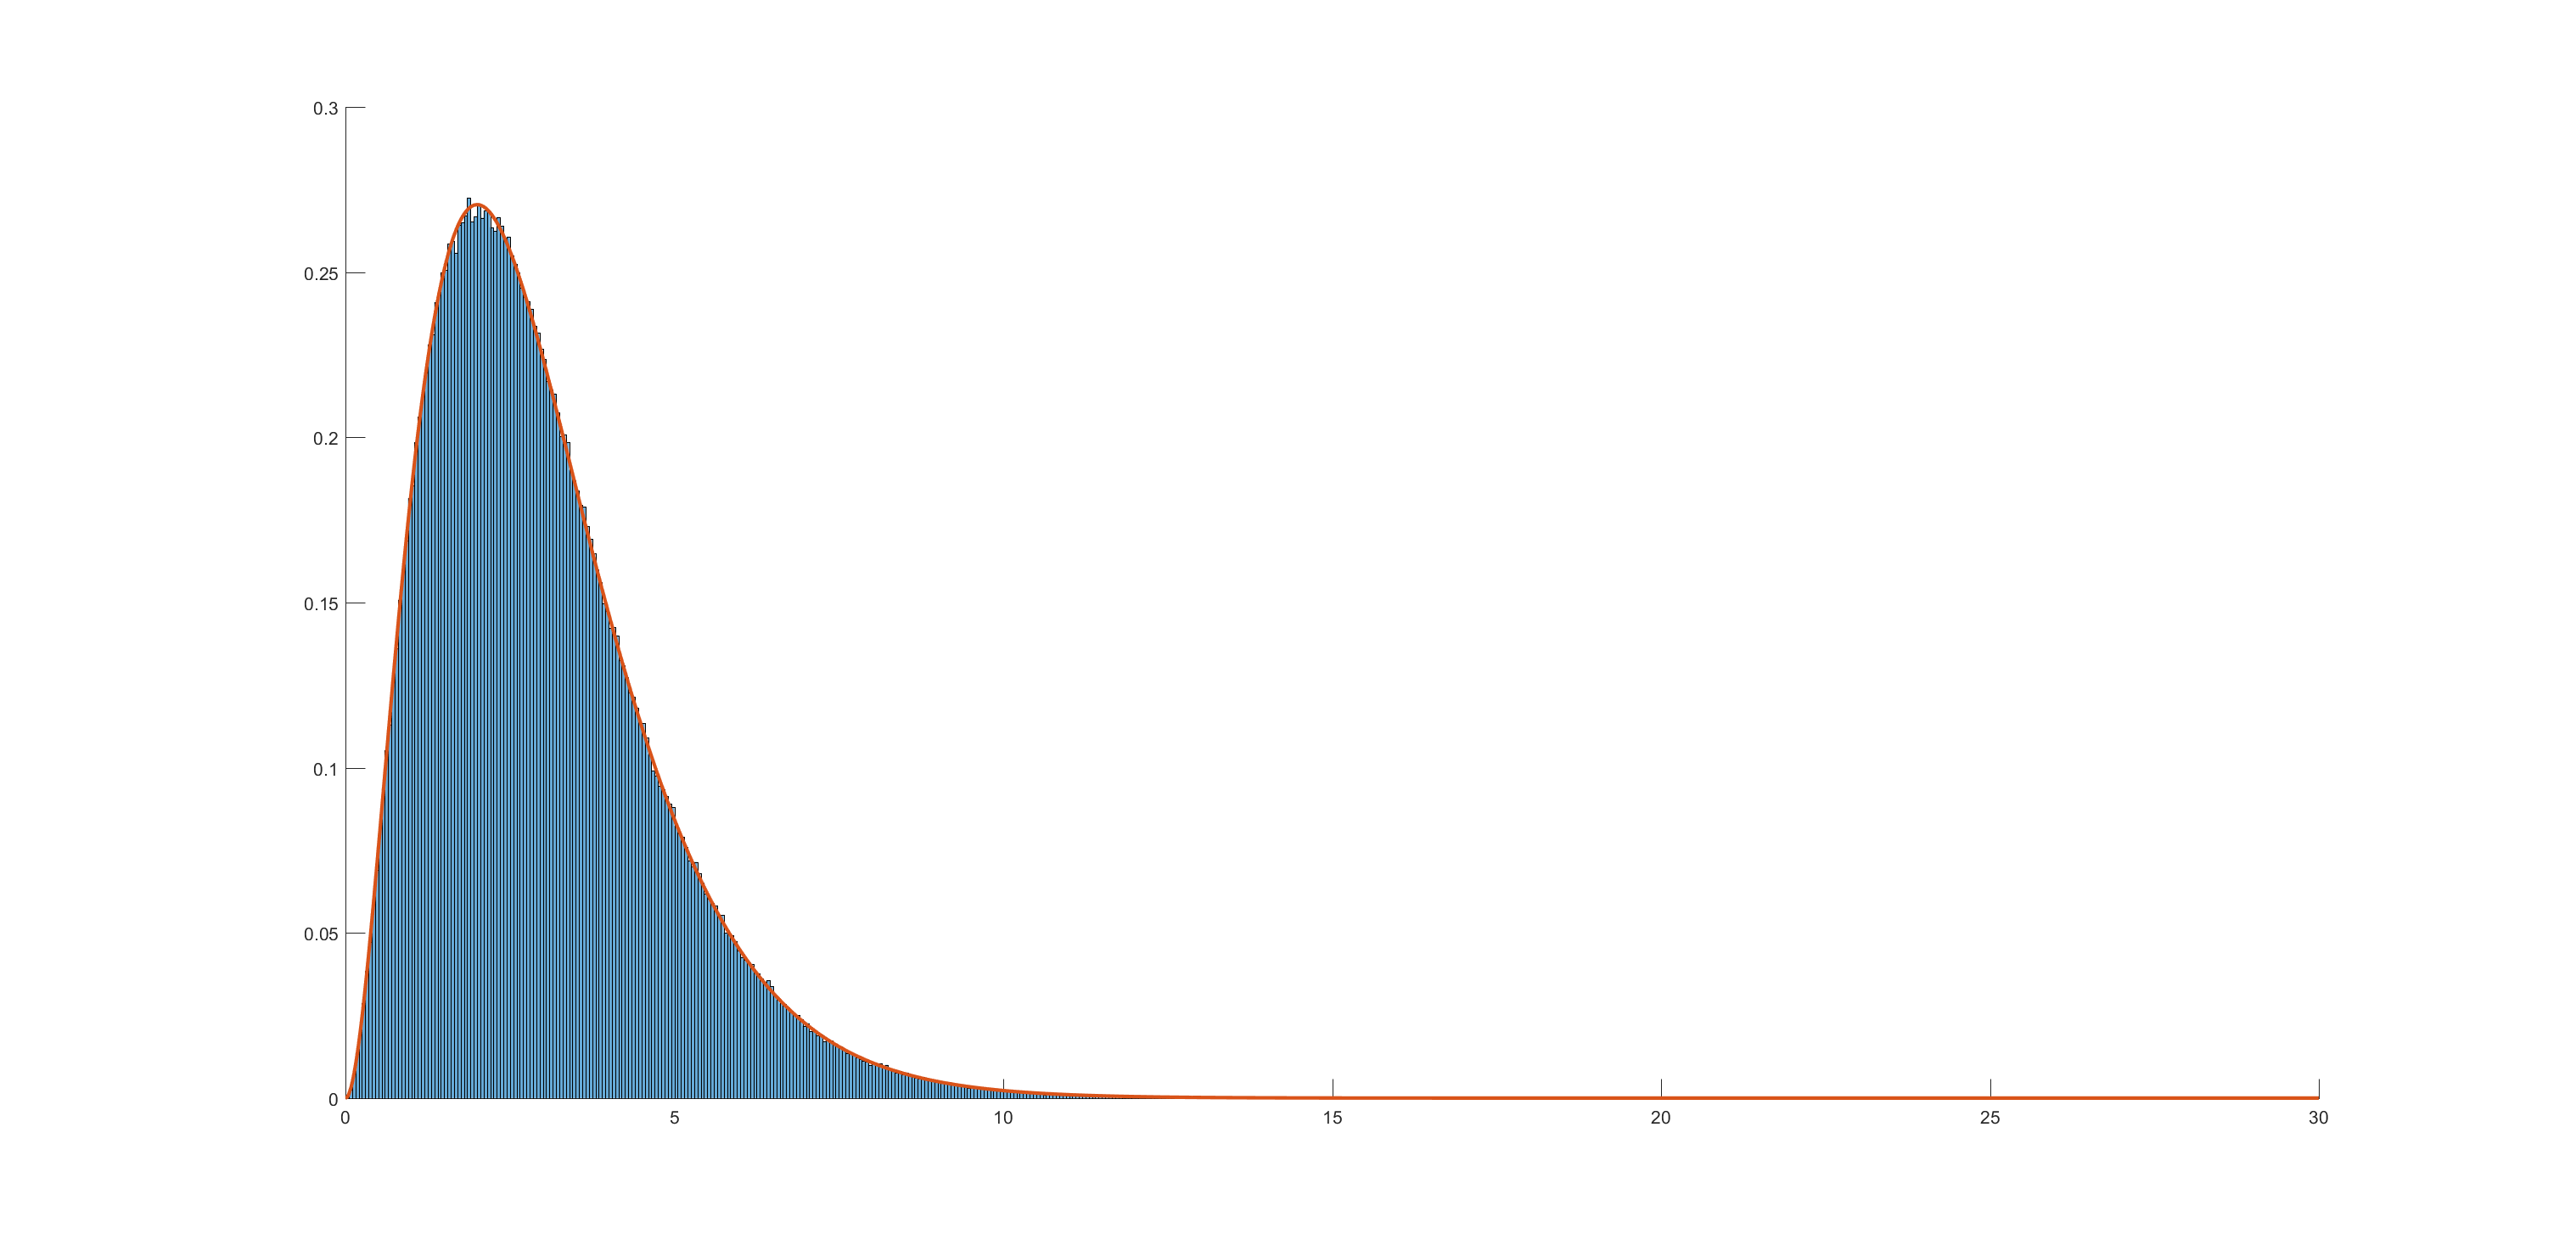
\includegraphics [width=\textwidth]{prob3_sim_03.eps}

\section{Problem 4}
\subsection{Results}
\begin{table}[h]
\centering
\caption{Descriptive Statistics for the Sample Means}
\label{p4_data}
\begin{tabular}{|l|l|l|l|l|l|l|l|}
  \hline 
n  & mean & variance & skewness & 0.025 quantile & 0.975 quantile & lower CI & upper CI \\
\hline
10 &1.0123& 0.10759  & 0.75211 & 0.4838 & 1.7838 & 0.30365 & 1.7209 \\
\hline
20 &1.0013& 0.051844 & 0.40566 & 0.60047 & 1.5232 & 0.50026 & 1.5024 \\
\hline
40 &1.0012& 0.025433 & 0.24374 & 0.71074 & 1.3243 & 0.64689 & 1.3555 \\
\hline
80 &1.0035& 0.013491 & 0.19314  & 0.7883 & 1.2431 & 0.75293 & 1.254 \\
\hline
\end{tabular}
\end{table}
\subsection{Discussion}
The Central Limit Theorem requires that a sample be sufficiently large for the distribution of the sample mean to be well approximated 
by the normal distribution. What constitutes a sufficiently large sample depends heavily on the shape and, more specifically,
the skewness of the population distribution. The exponential distribution used in this example is highly skewed which
means more samples will be needed to closely approximate the distribution of the sample means with the normal distribution than if the
population distribution more closely resembled a normal distribution itself. This can be seen particularly well by observing the skewness
of the sample means. As the number of samples in each group gets large the skewness asymptotically approaches zero, which is the value of
skewness for a normal distribution. The CLT clearly doesn't hold for samples of size 10. The lower confidence interval is much too
conservative and the upper confidence interval is anti-conservative. The CLT is a better approximation for samples of size 20, but the
upper bound of the confidence interval is still anti-conservative. The CLT begins to hold up for samples of size 40. The quantiles are
closely approximated by the confidence intervals predicted by the CLT and both are conservative estimates. Obviously the CLT holds for
sample sizes of 80, but what's disconcerting is how little the skewness decreases compared to the value at 40 samples. Since this 
value controls just how good an approximation the CLT provides it's unfortunate that it will take a huge number of additional 
samples to make the approximation better. This is illustrated better by the figures below. Additional sample sizes were explored 
that show the small effect large samples have on skewness for highly skewed distributions. Overall, the CLT is a great tool, but 
care must be taken to ensure that the approximation holds up in practice.
\subsection*{Contents}

\begin{itemize}
\setlength{\itemsep}{-1ex}
   \item Final Problem 4
   \item A. Generate the population of Gamma RVs
   \item B Part 1: Create Sample Distributions of Size n
\end{itemize}


\subsection*{Final Problem 4}

\begin{par}
Taylor Bodin 9 Dec 2016
\end{par} \vspace{1em}
\begin{verbatim}
% Setup Variables
clear; close all; clc;
set(0,'DefaultFigureWindowStyle','docked')

N = 500000; %Number of RV in the population
num_bins = 50; %Standard number of bins for histograms
n = [10 20 40 80 100 200 500];
ci = .975;
\end{verbatim}


\subsection*{A: Generate the population of Gamma RVs}

\begin{verbatim}
pop = random('Gamma',1,1,[1,N]);

% Descripitive Stats
mu = mean(pop); % Given
var = std(pop)^2;
skew = skewness(pop);
pop_quant_upper = quantile(pop,ci);
pop_quant_lower = quantile(pop,1-ci);

pop_stat_str = {['\mu = ', num2str(mu)];
    ['\sigma^2 = ' num2str(var)];
    ['Skew = ' num2str(skew)];
    ['Upper Quantile: ' num2str(pop_quant_upper)];
    ['Lower Quantile: ' num2str(pop_quant_lower)]};


% Population Figure
f1 = figure(1);

% Histogram
pop_hist = histogram(pop);
pop_hist.Normalization = 'PDF';
pop_hist.NumBins = num_bins;

% Quantiles
line([pop_quant_lower pop_quant_lower], get(gca, 'ylim'),...
    'Color', 'Red', 'LineWidth', 2, 'LineStyle', '--');
line([pop_quant_upper pop_quant_upper], get(gca, 'ylim'),...
    'Color', 'Green', 'LineWidth', 2, 'LineStyle', '--');

% Annotation
dim = [.4 .3 .3 .3];
annotation('textbox',dim,'String',pop_stat_str,'FitBoxToText','on');

% Figure Properties
title('Simulated PDF of the Gamma(1,1) RV')
xlabel('RV value');
f1.CurrentAxes.XAxis.Limits = [0 4];
ylabel('Probability Density');
legend('Gamma(1,1) PDF', 'Lower Quantile (.025)', 'Upper Quantile (.975)');
\end{verbatim}

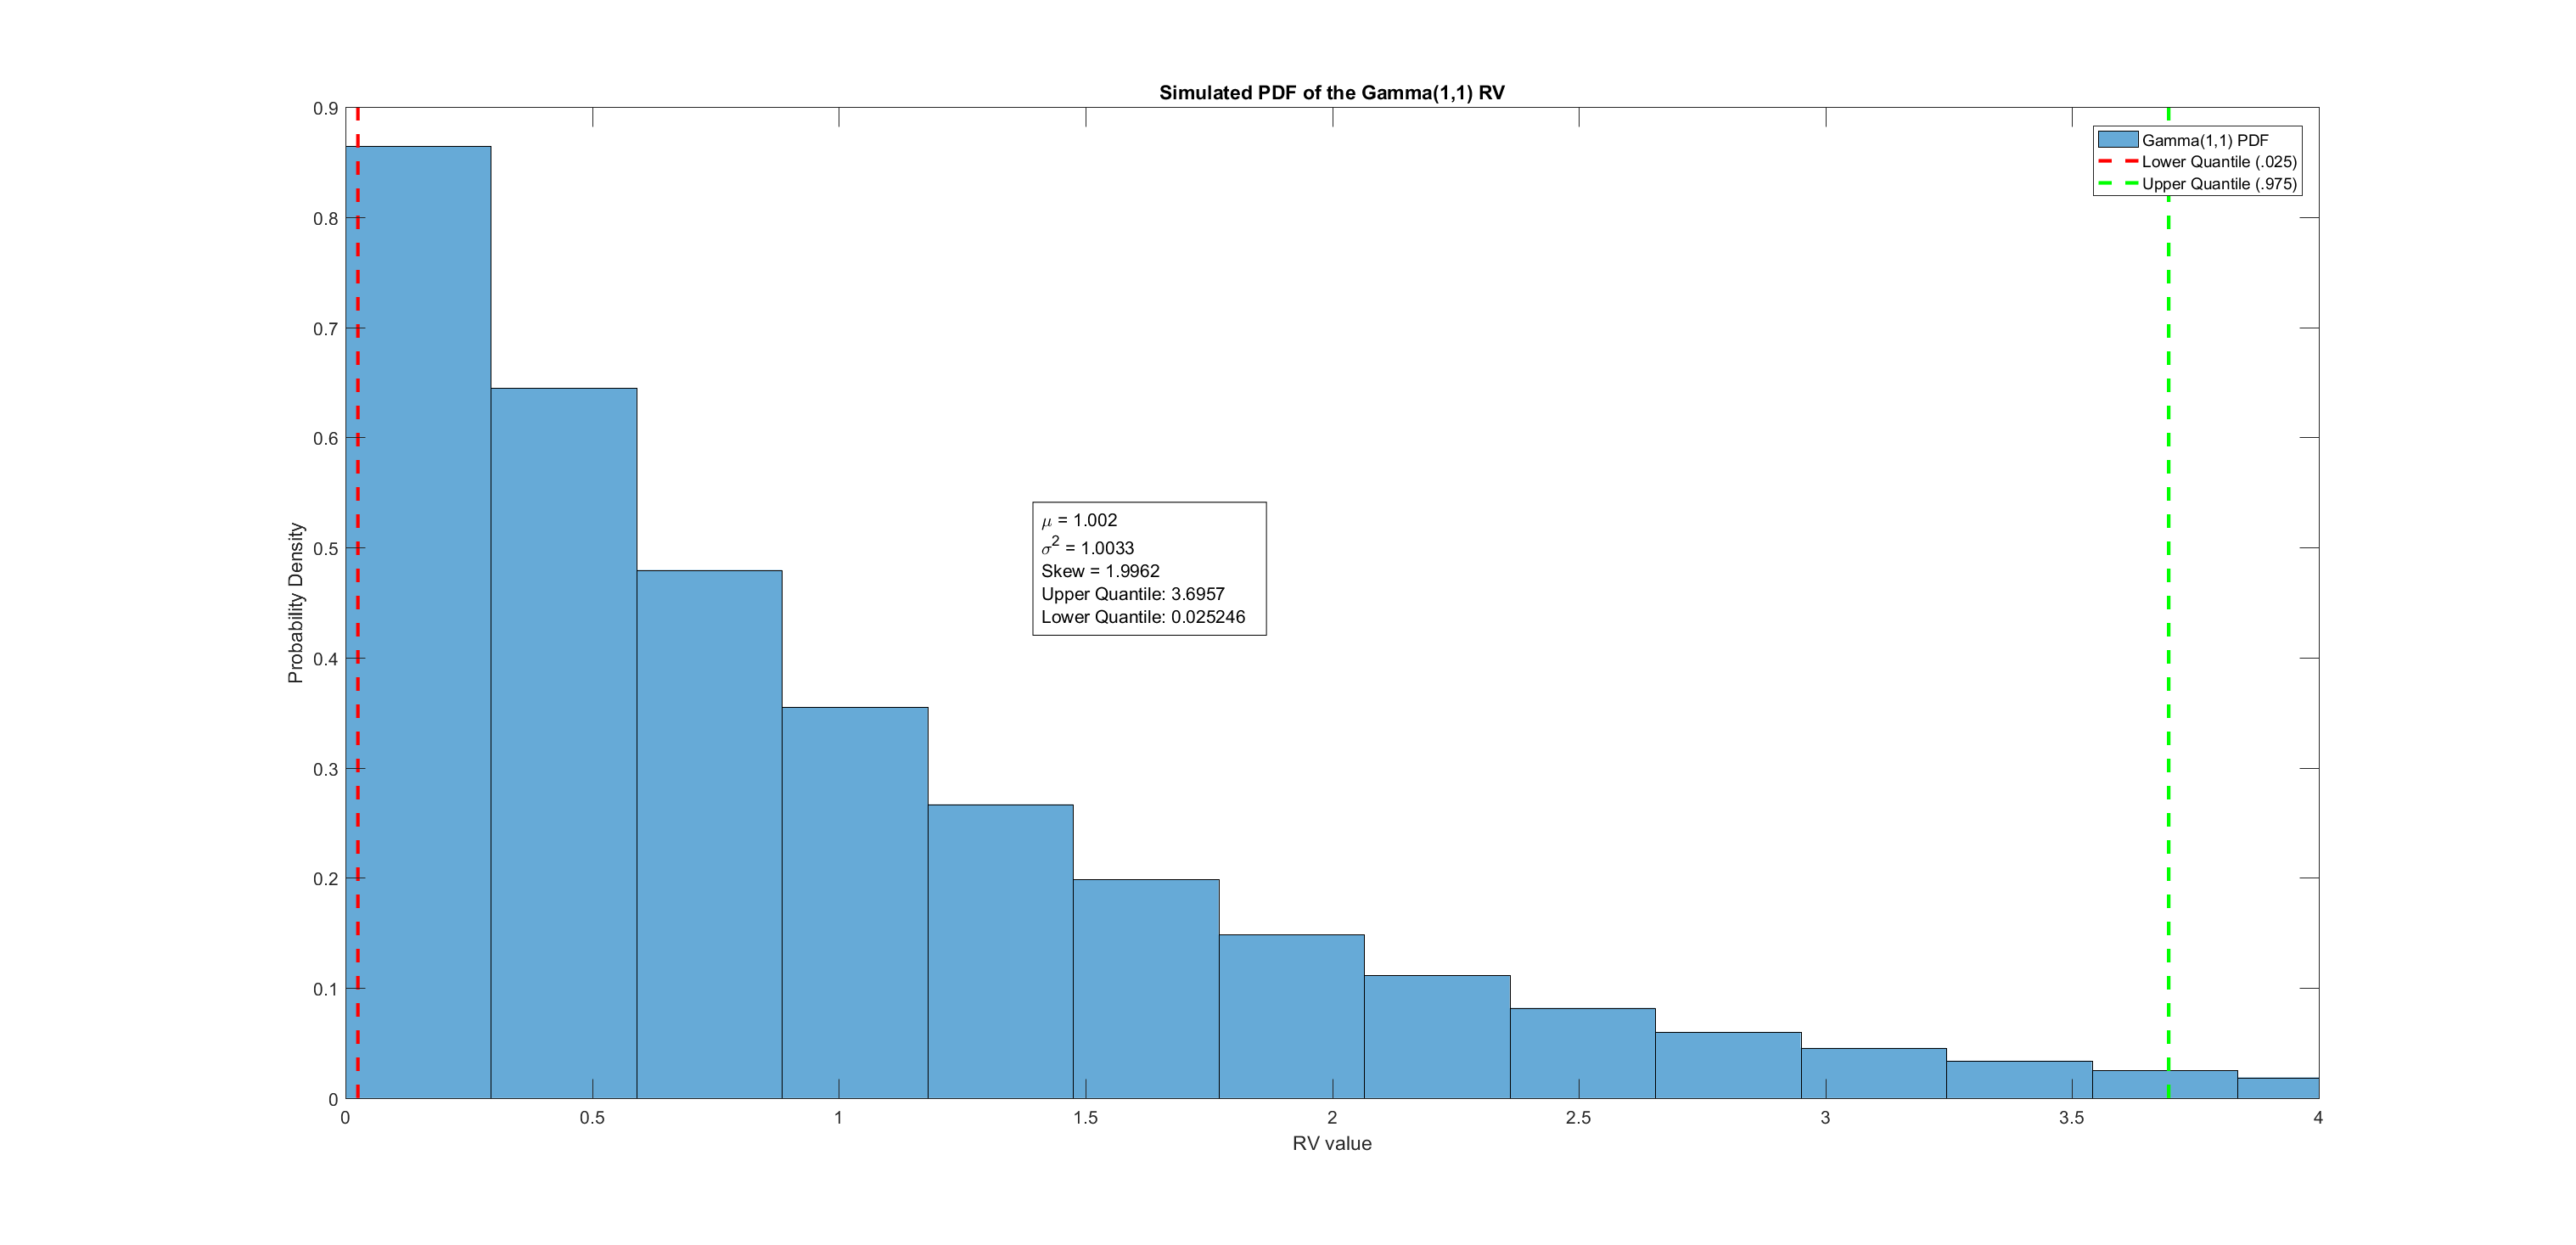
\includegraphics [width=\textwidth]{prob4_01.eps}


\subsection*{B: Create Sample Distributions of Size n}

\begin{verbatim}
for k=1:length(n)

sample = reshape(pop,n(k),[]);
sample = sample(:,1:1000); % Per the instructions only want 1000

% Descriptive Stats
s_mu = mean(sample);
mu_var = mean(std(s_mu).^2);
mu_skew = mean(skewness(s_mu));
s_quant_upper = mean(quantile(s_mu,ci));
s_quant_lower = mean(quantile(s_mu,1-ci));
ci_upper = mean(s_mu + sqrt(var/n(k))*qfuncinv((1-ci)/2));
ci_lower = mean(s_mu - sqrt(var/n(k))*qfuncinv((1-ci)/2));

% Summary of Descriptive Stats
s_stat_str = {['\mu = ', num2str(mean(s_mu))];
    ['\sigma^2 = ' num2str(mu_var)];
    ['Skew = ' num2str(mu_skew)];
    ['Upper Quantile: ' num2str(s_quant_upper)];
    ['Lower Quantile: ' num2str(s_quant_lower)];
    ['Upper Confidence Interval: ' num2str(ci_upper)];
    ['Lower Confidence Interval: ' num2str(ci_lower)]};


% Central Limit Theorem Approximation
cl_pd = makedist('Normal', 'mu', mu, 'sigma', var/sqrt(n(k)));
range = 0:.01:2.5;
cl_pdf = pdf(cl_pd,range);

% Create the figure
f2 = figure(k+1);
hold on
% -- Mean Histogram
s_hist = histogram(s_mu);
s_hist.Normalization = 'PDF';
s_hist.NumBins = num_bins;

xlims = f2.CurrentAxes.XAxis.Limits; %Need these xlims scaled for the hist

% -- Quantiles
q1 = line([s_quant_lower s_quant_lower], get(gca, 'ylim'),...
    'Color', 'Green', 'LineWidth', 2, 'LineStyle', '--');
q2 = line([s_quant_upper s_quant_upper], get(gca, 'ylim'),...
    'Color', 'Green', 'LineWidth', 2, 'LineStyle', '--');

% -- Central Limit Approximation
p1 = plot(range,cl_pdf, 'LineWidth', 2, 'LineStyle', '-.');

% -- Confidence Intervals
ci_1 = line([ci_lower ci_lower], get(gca, 'ylim'),...
    'Color', 'Red', 'LineWidth', 2, 'LineStyle', '--');
ci_2 = line([ci_upper ci_upper], get(gca, 'ylim'),...
    'Color', 'Red', 'LineWidth', 2, 'LineStyle', '--');

% -- Descripitve Annotation
dim = [.815 .52 .3 .3];
a1 = annotation('textbox',dim,'String',s_stat_str,'FitBoxToText','on');

% -- Figure Properties
f2.CurrentAxes.XAxis.Limits = xlims;
title(['PDF of Sample Means of Sample Size ' num2str(n(k))])
xlabel('Value of \mu');
ylabel('Probability Density');
legend([s_hist q1 p1 ci_1], ...
    ['PDF of \mu_{N=' num2str(n(k)) '}'], '97.5% Quantiles'...
    ,'Central Limit Approximation', '97.5% Confidence Intervals');
hold off
end
\end{verbatim}

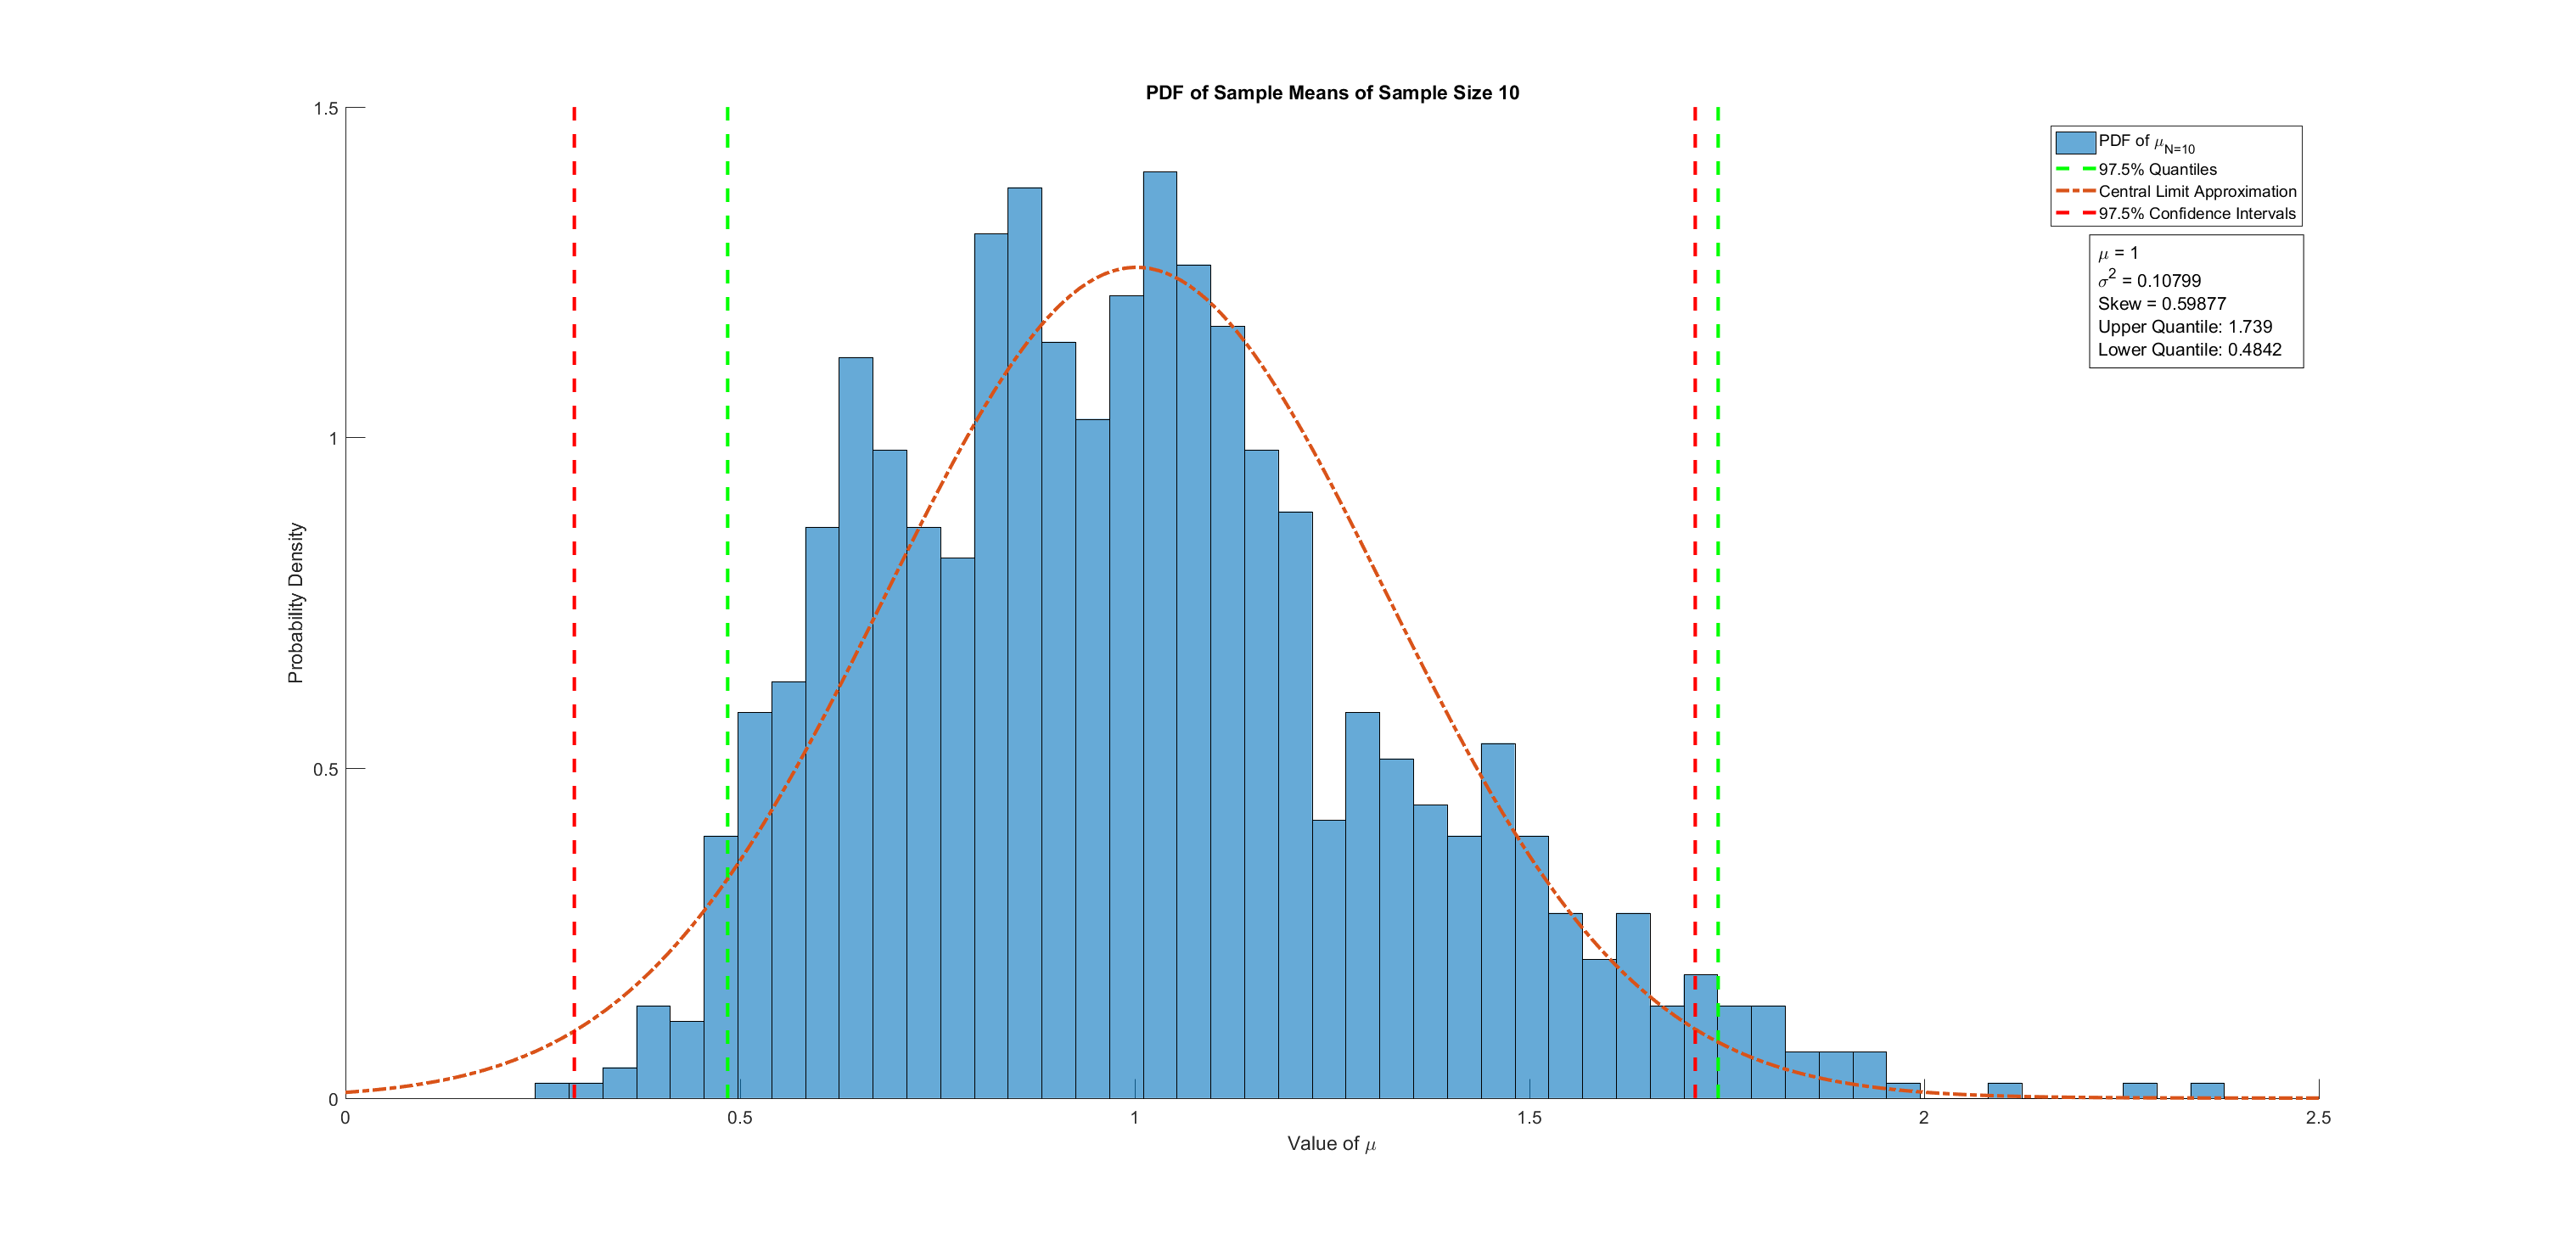
\includegraphics [width=\textwidth]{prob4_02.eps}

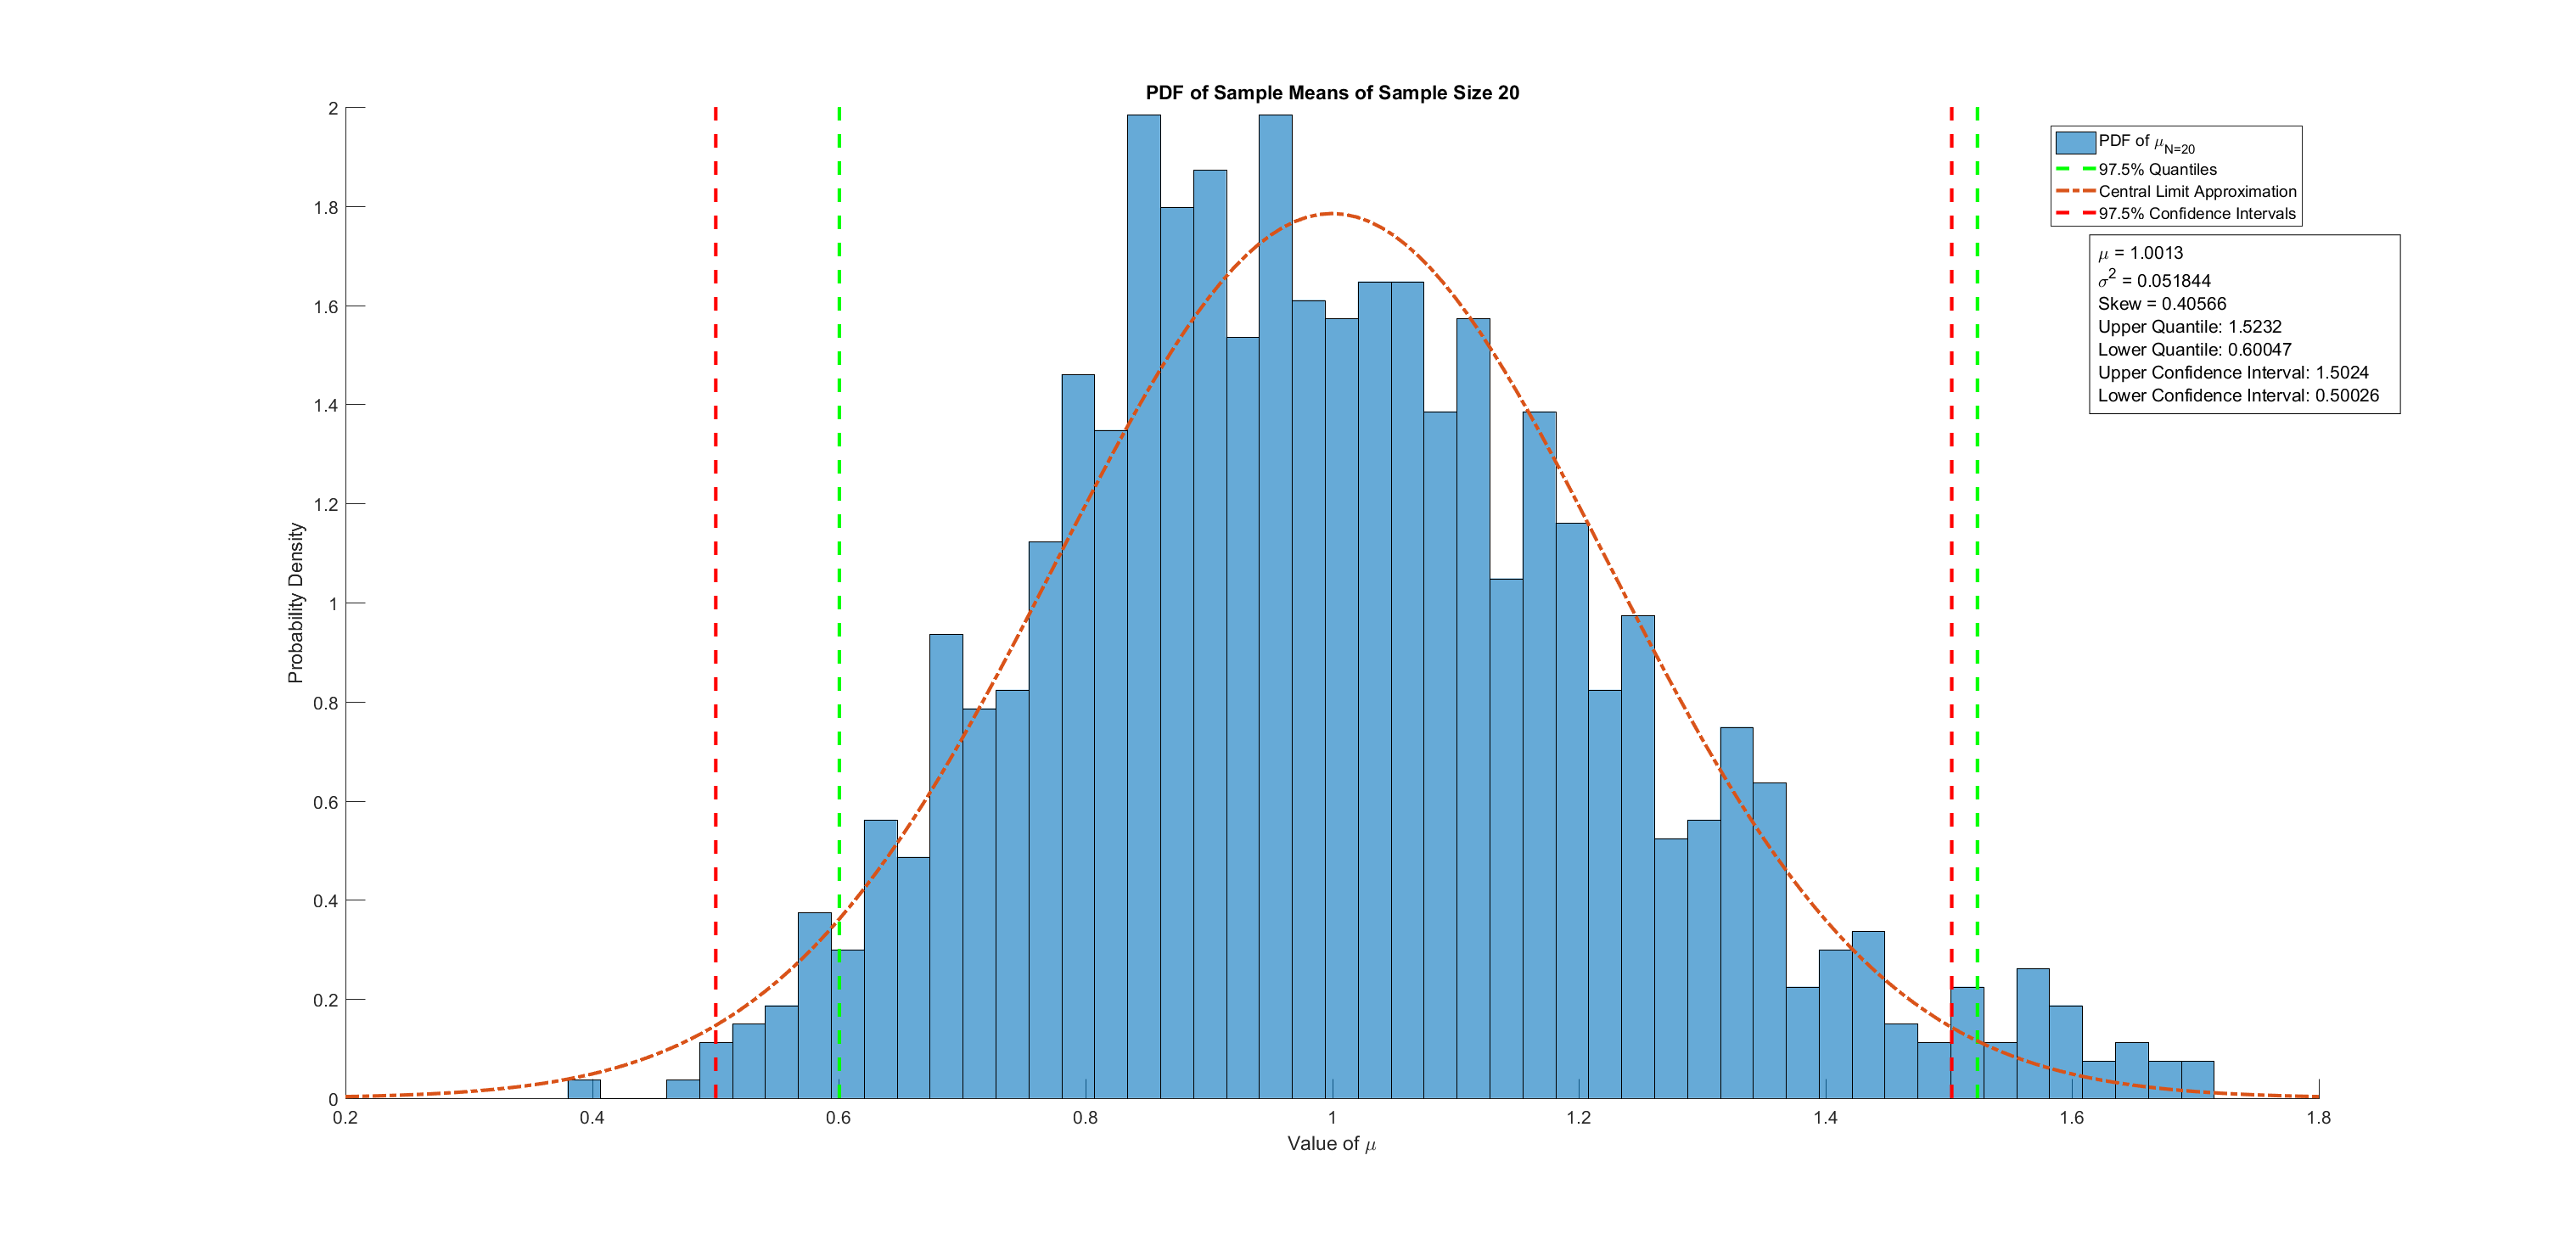
\includegraphics [width=\textwidth]{prob4_03.eps}

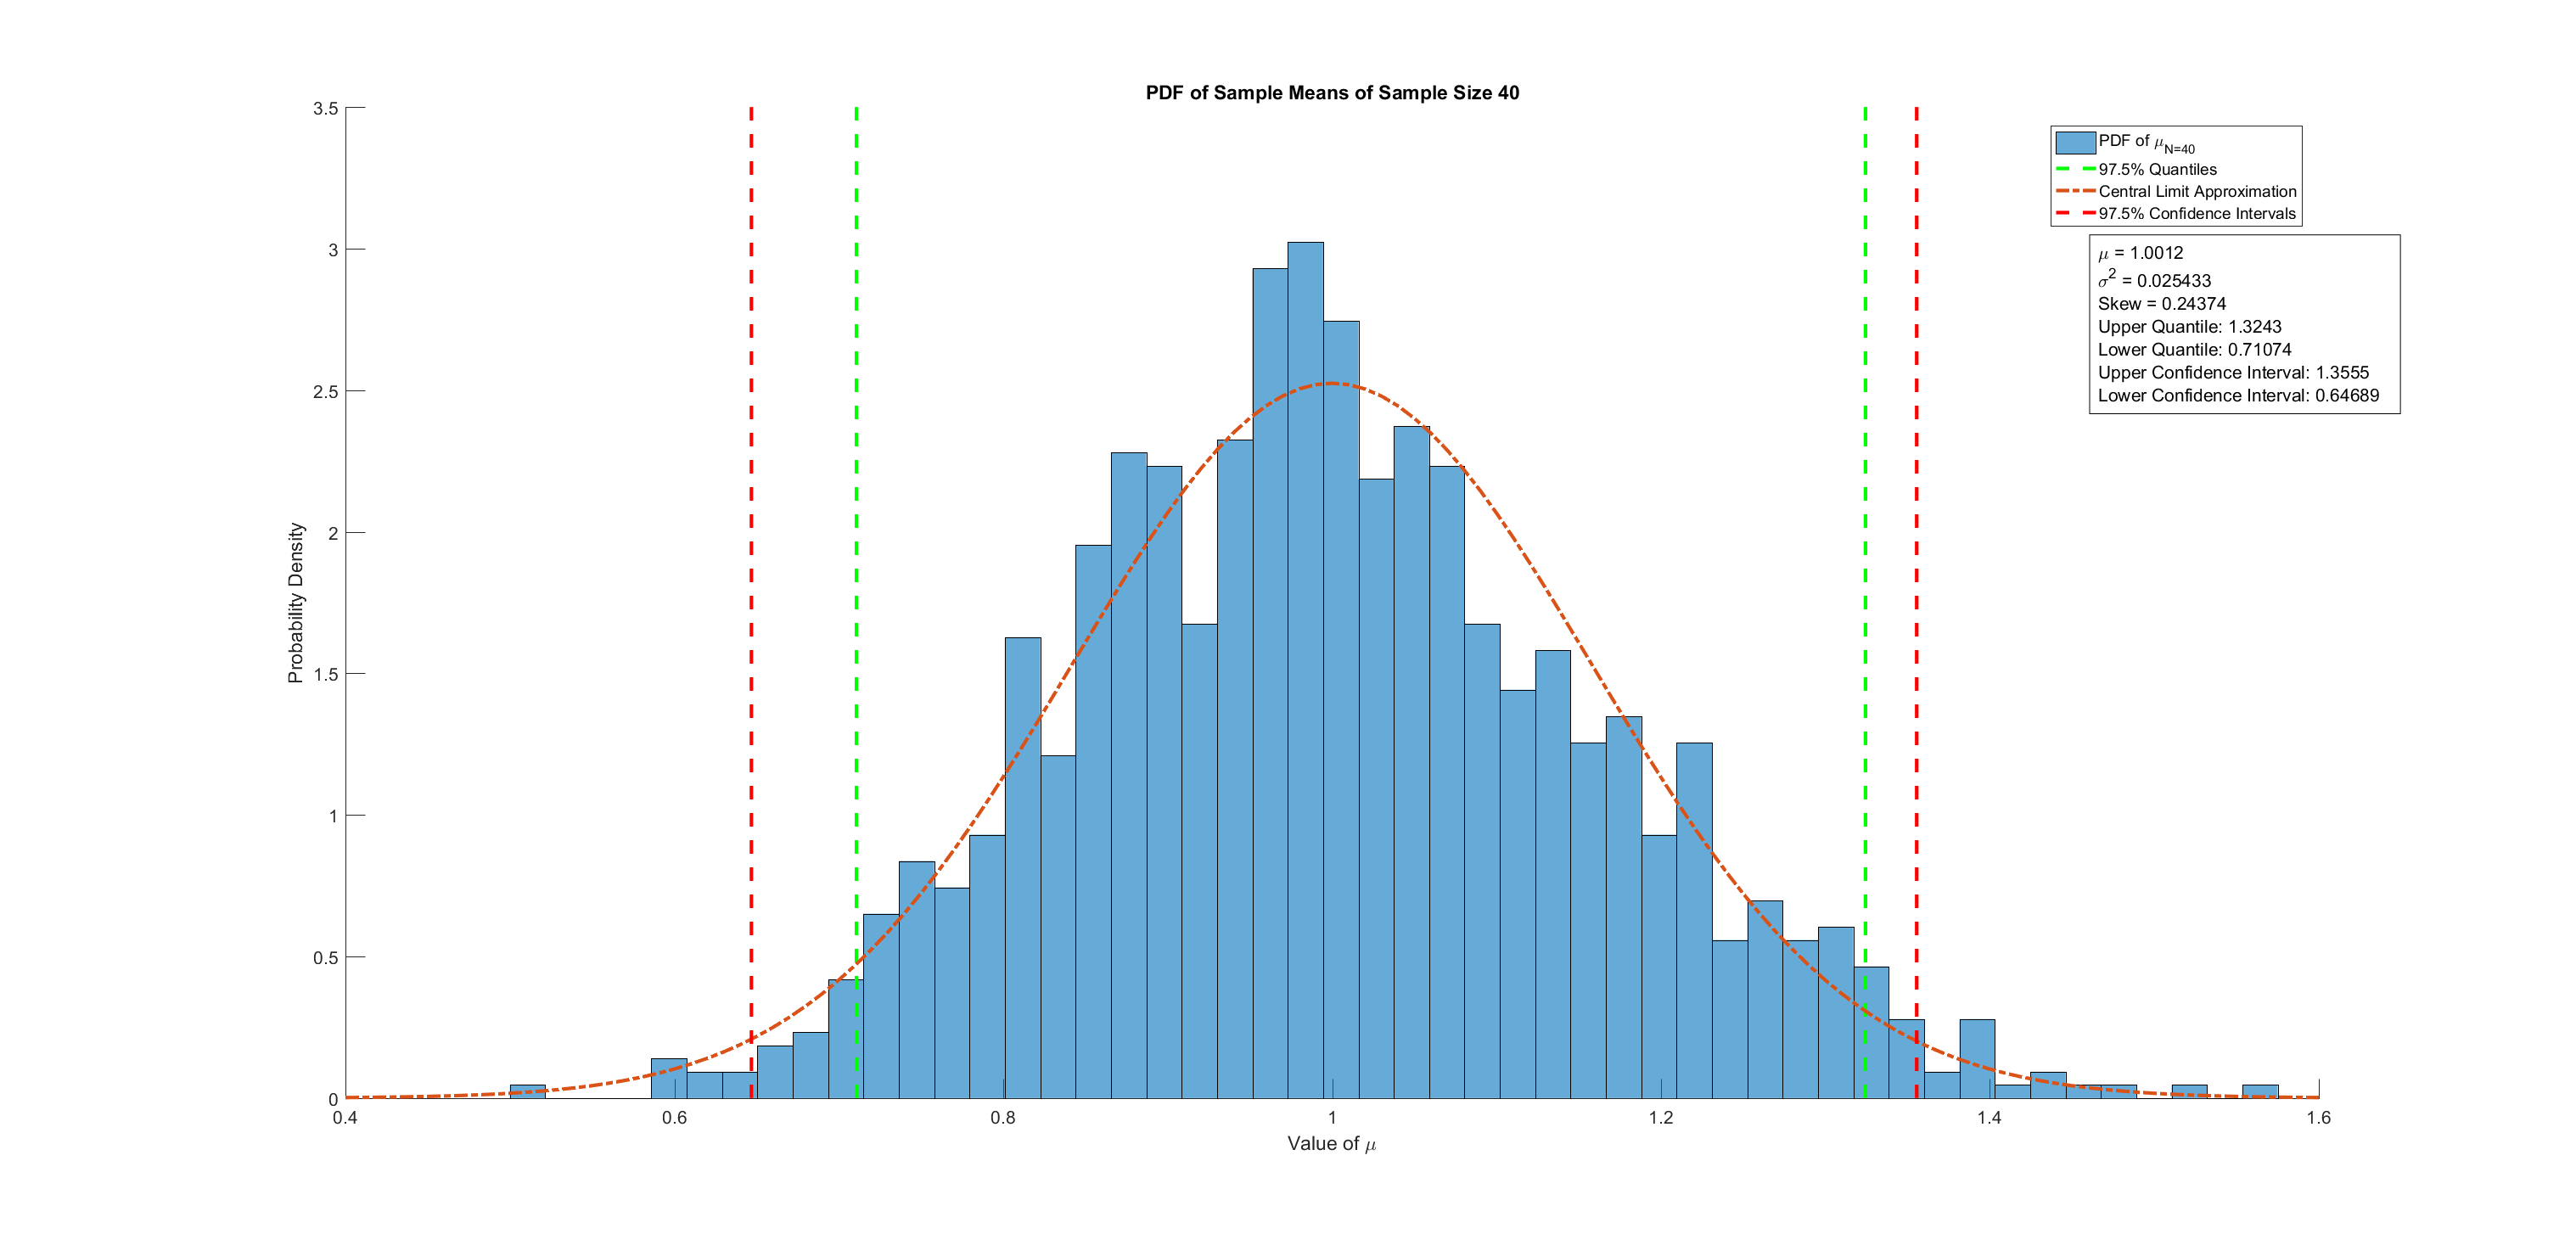
\includegraphics [width=\textwidth]{prob4_04.eps}

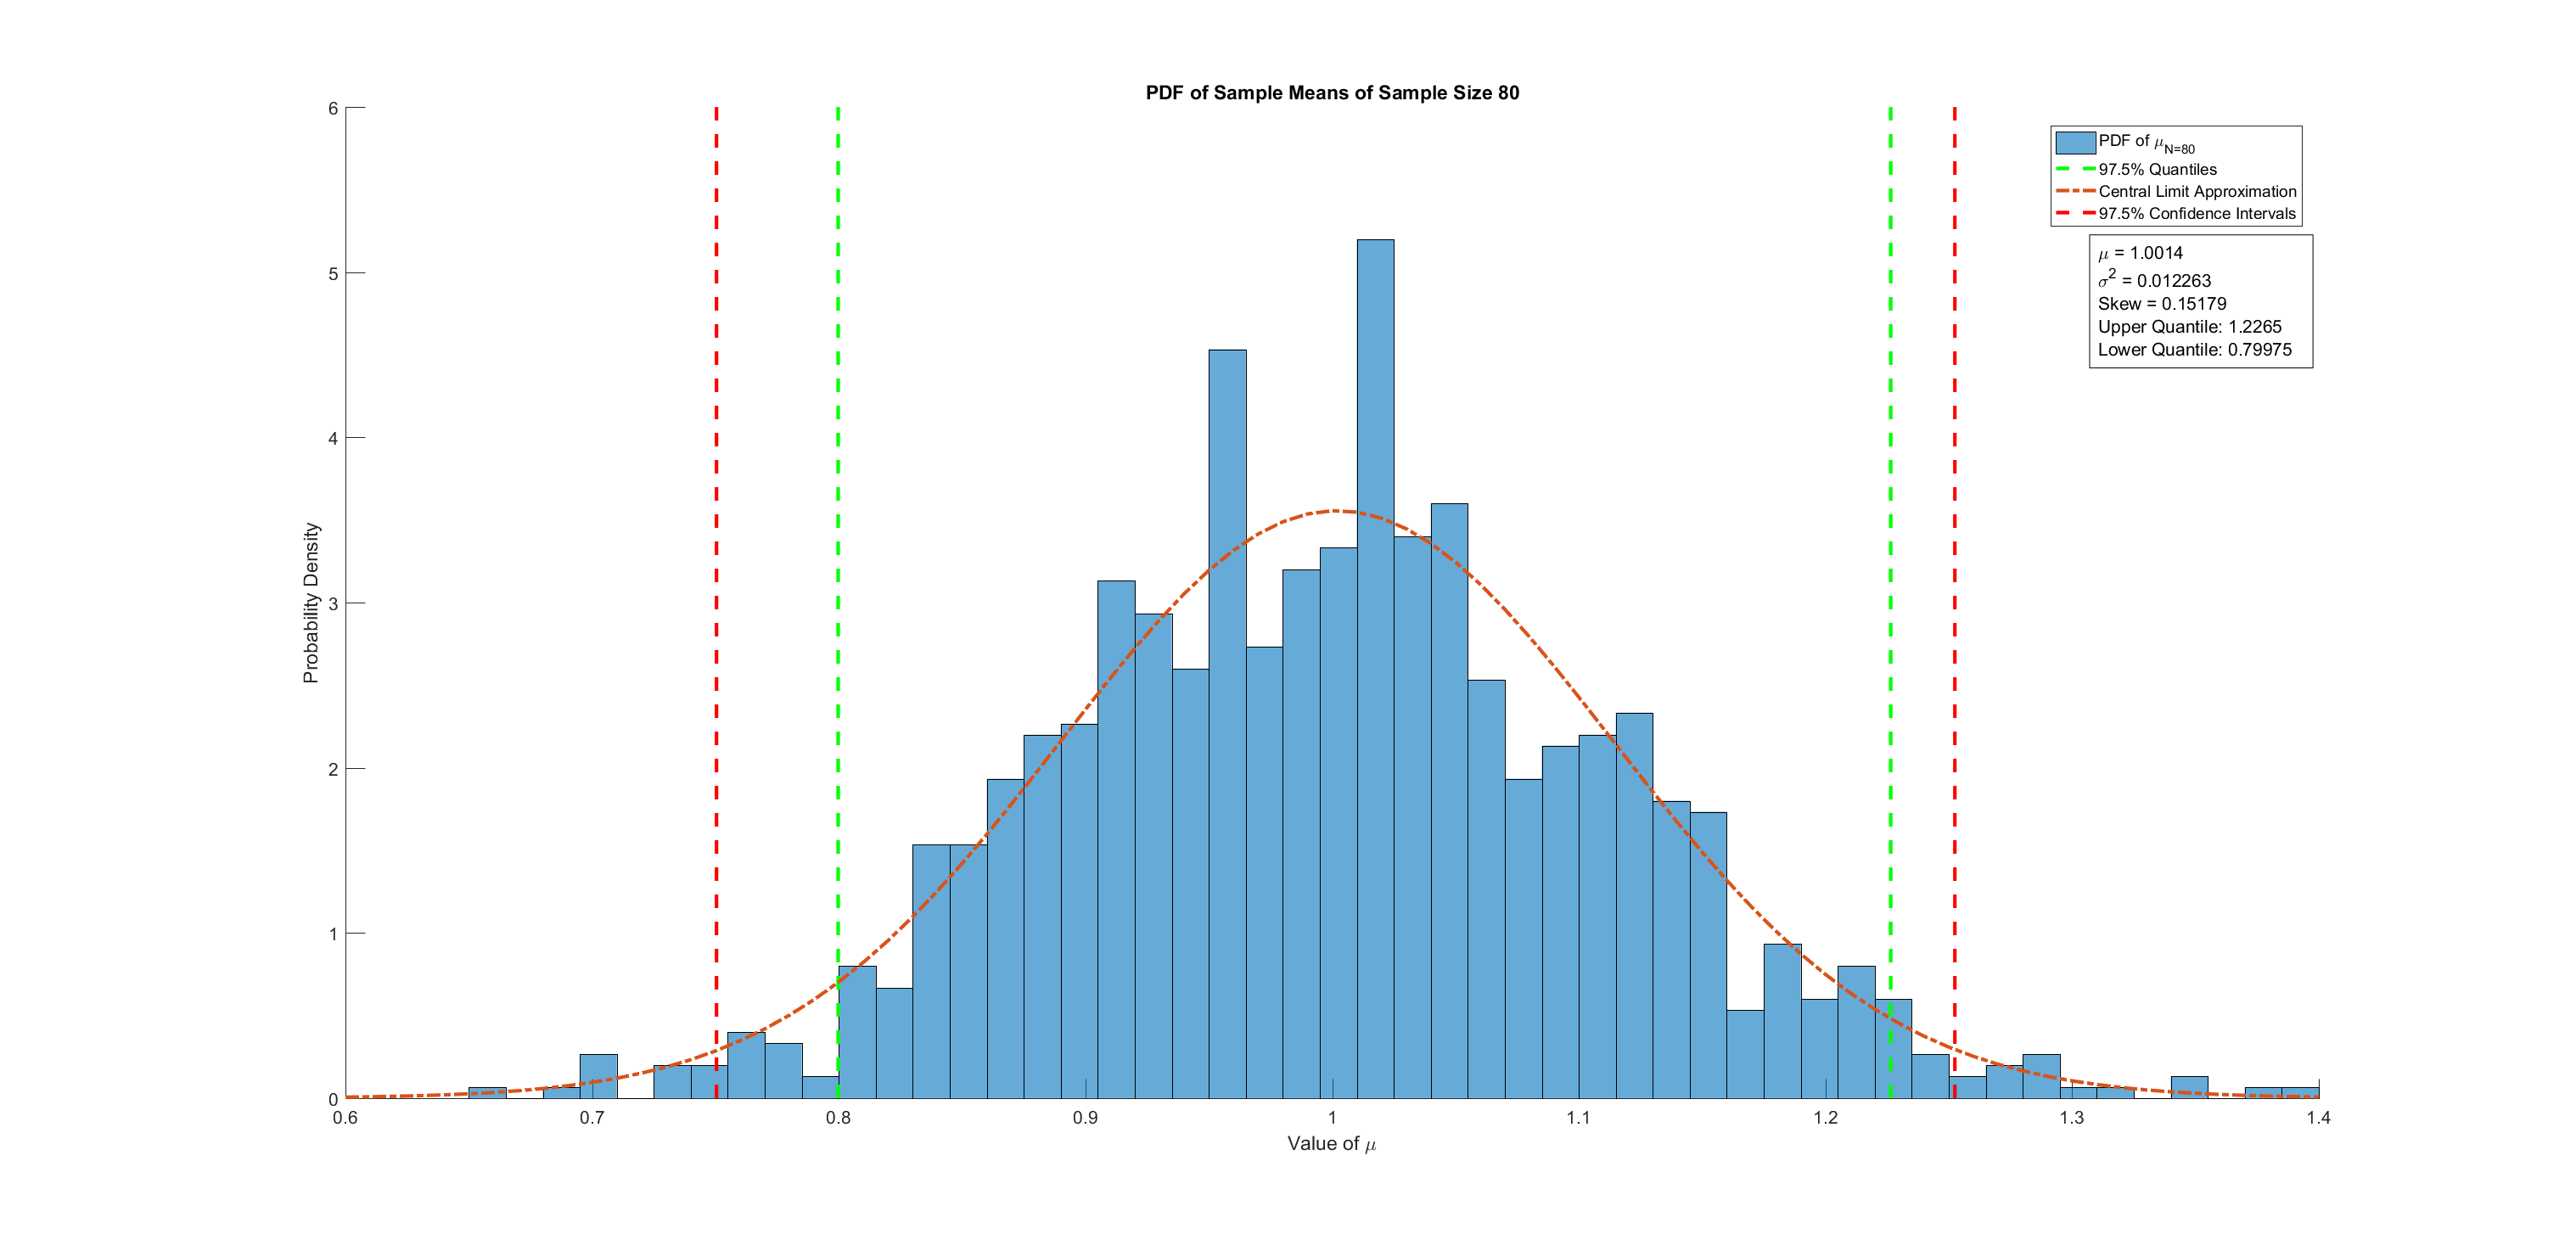
\includegraphics [width=\textwidth]{prob4_05.eps}

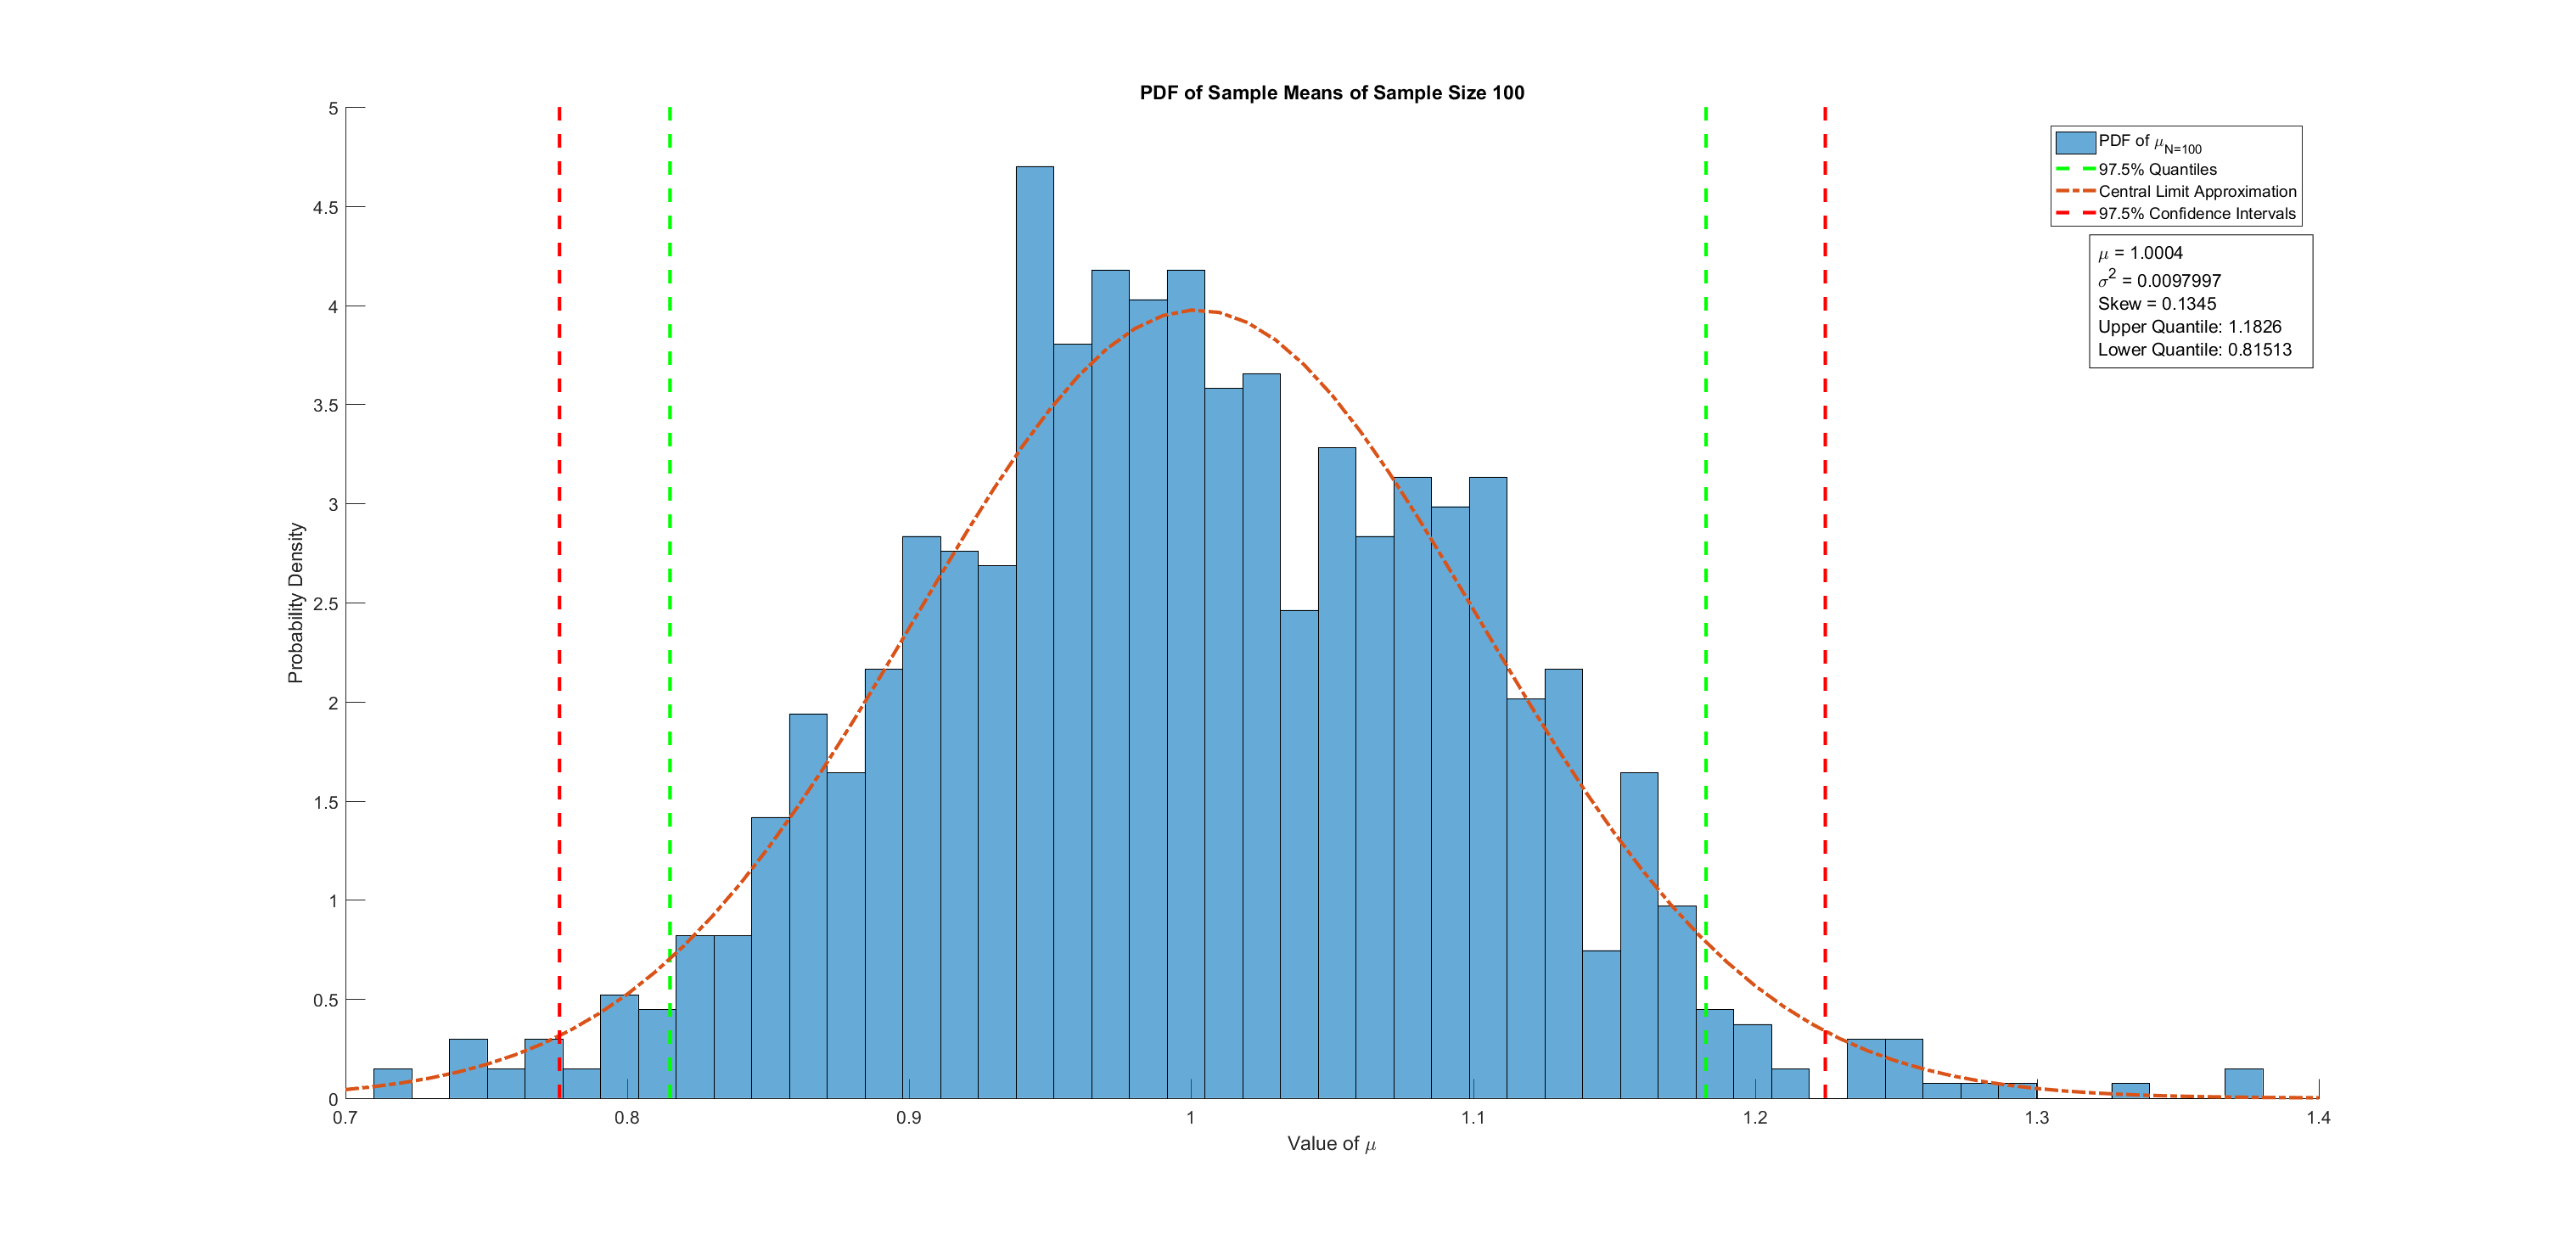
\includegraphics [width=\textwidth]{prob4_06.eps}

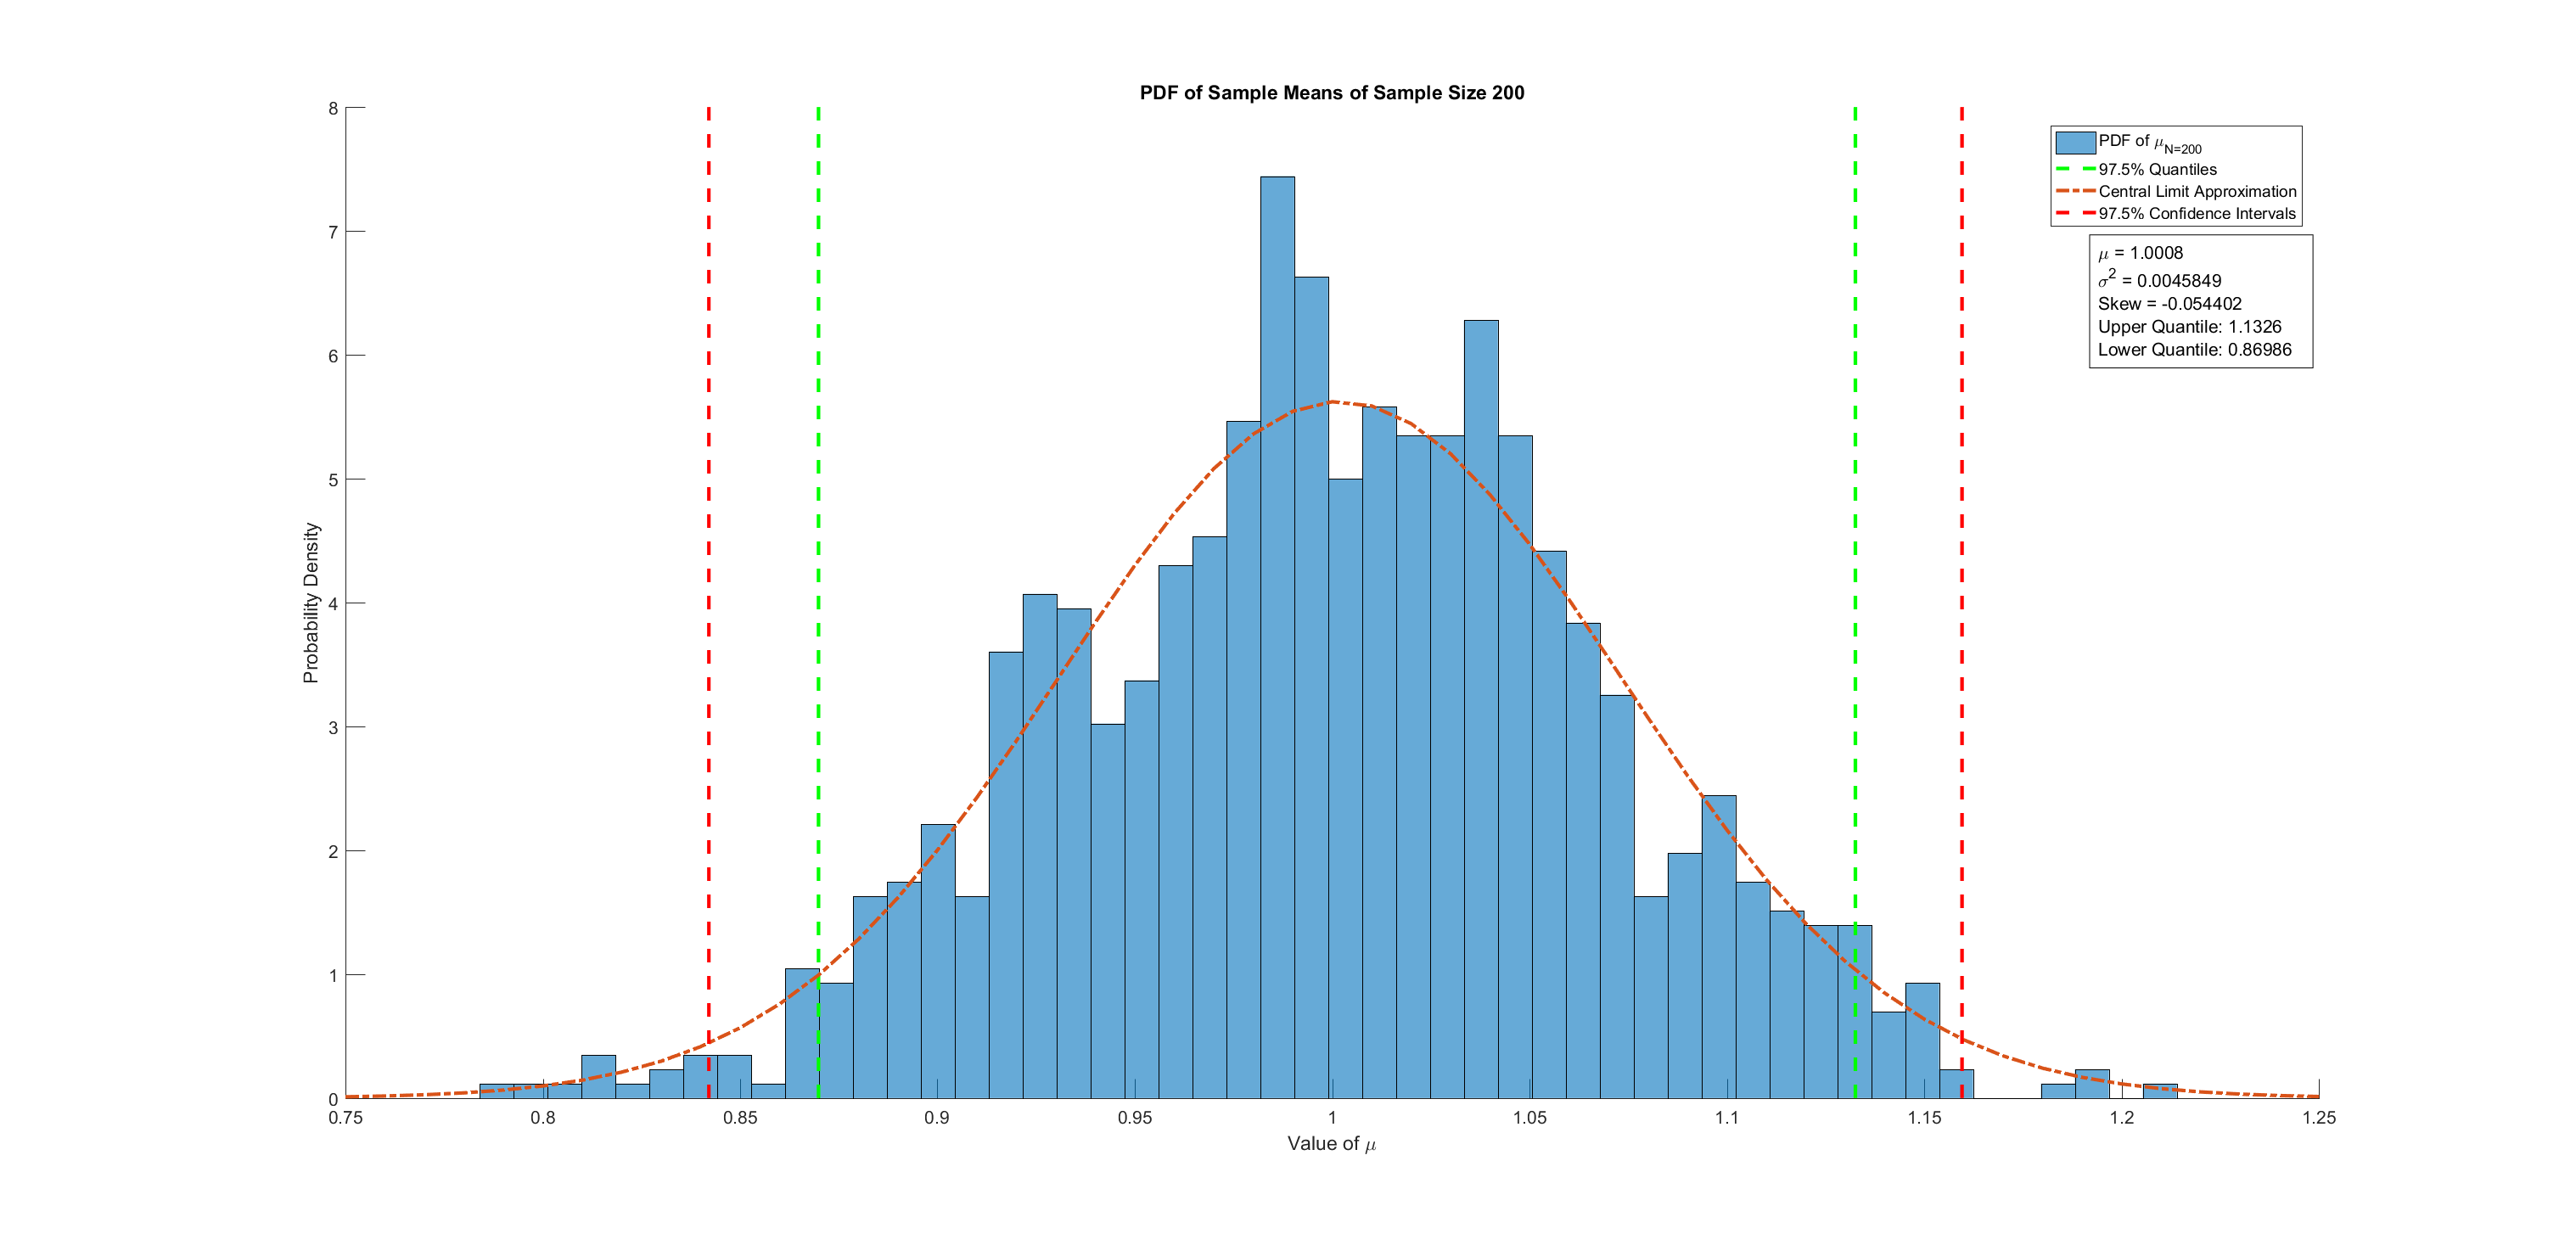
\includegraphics [width=\textwidth]{prob4_07.eps}

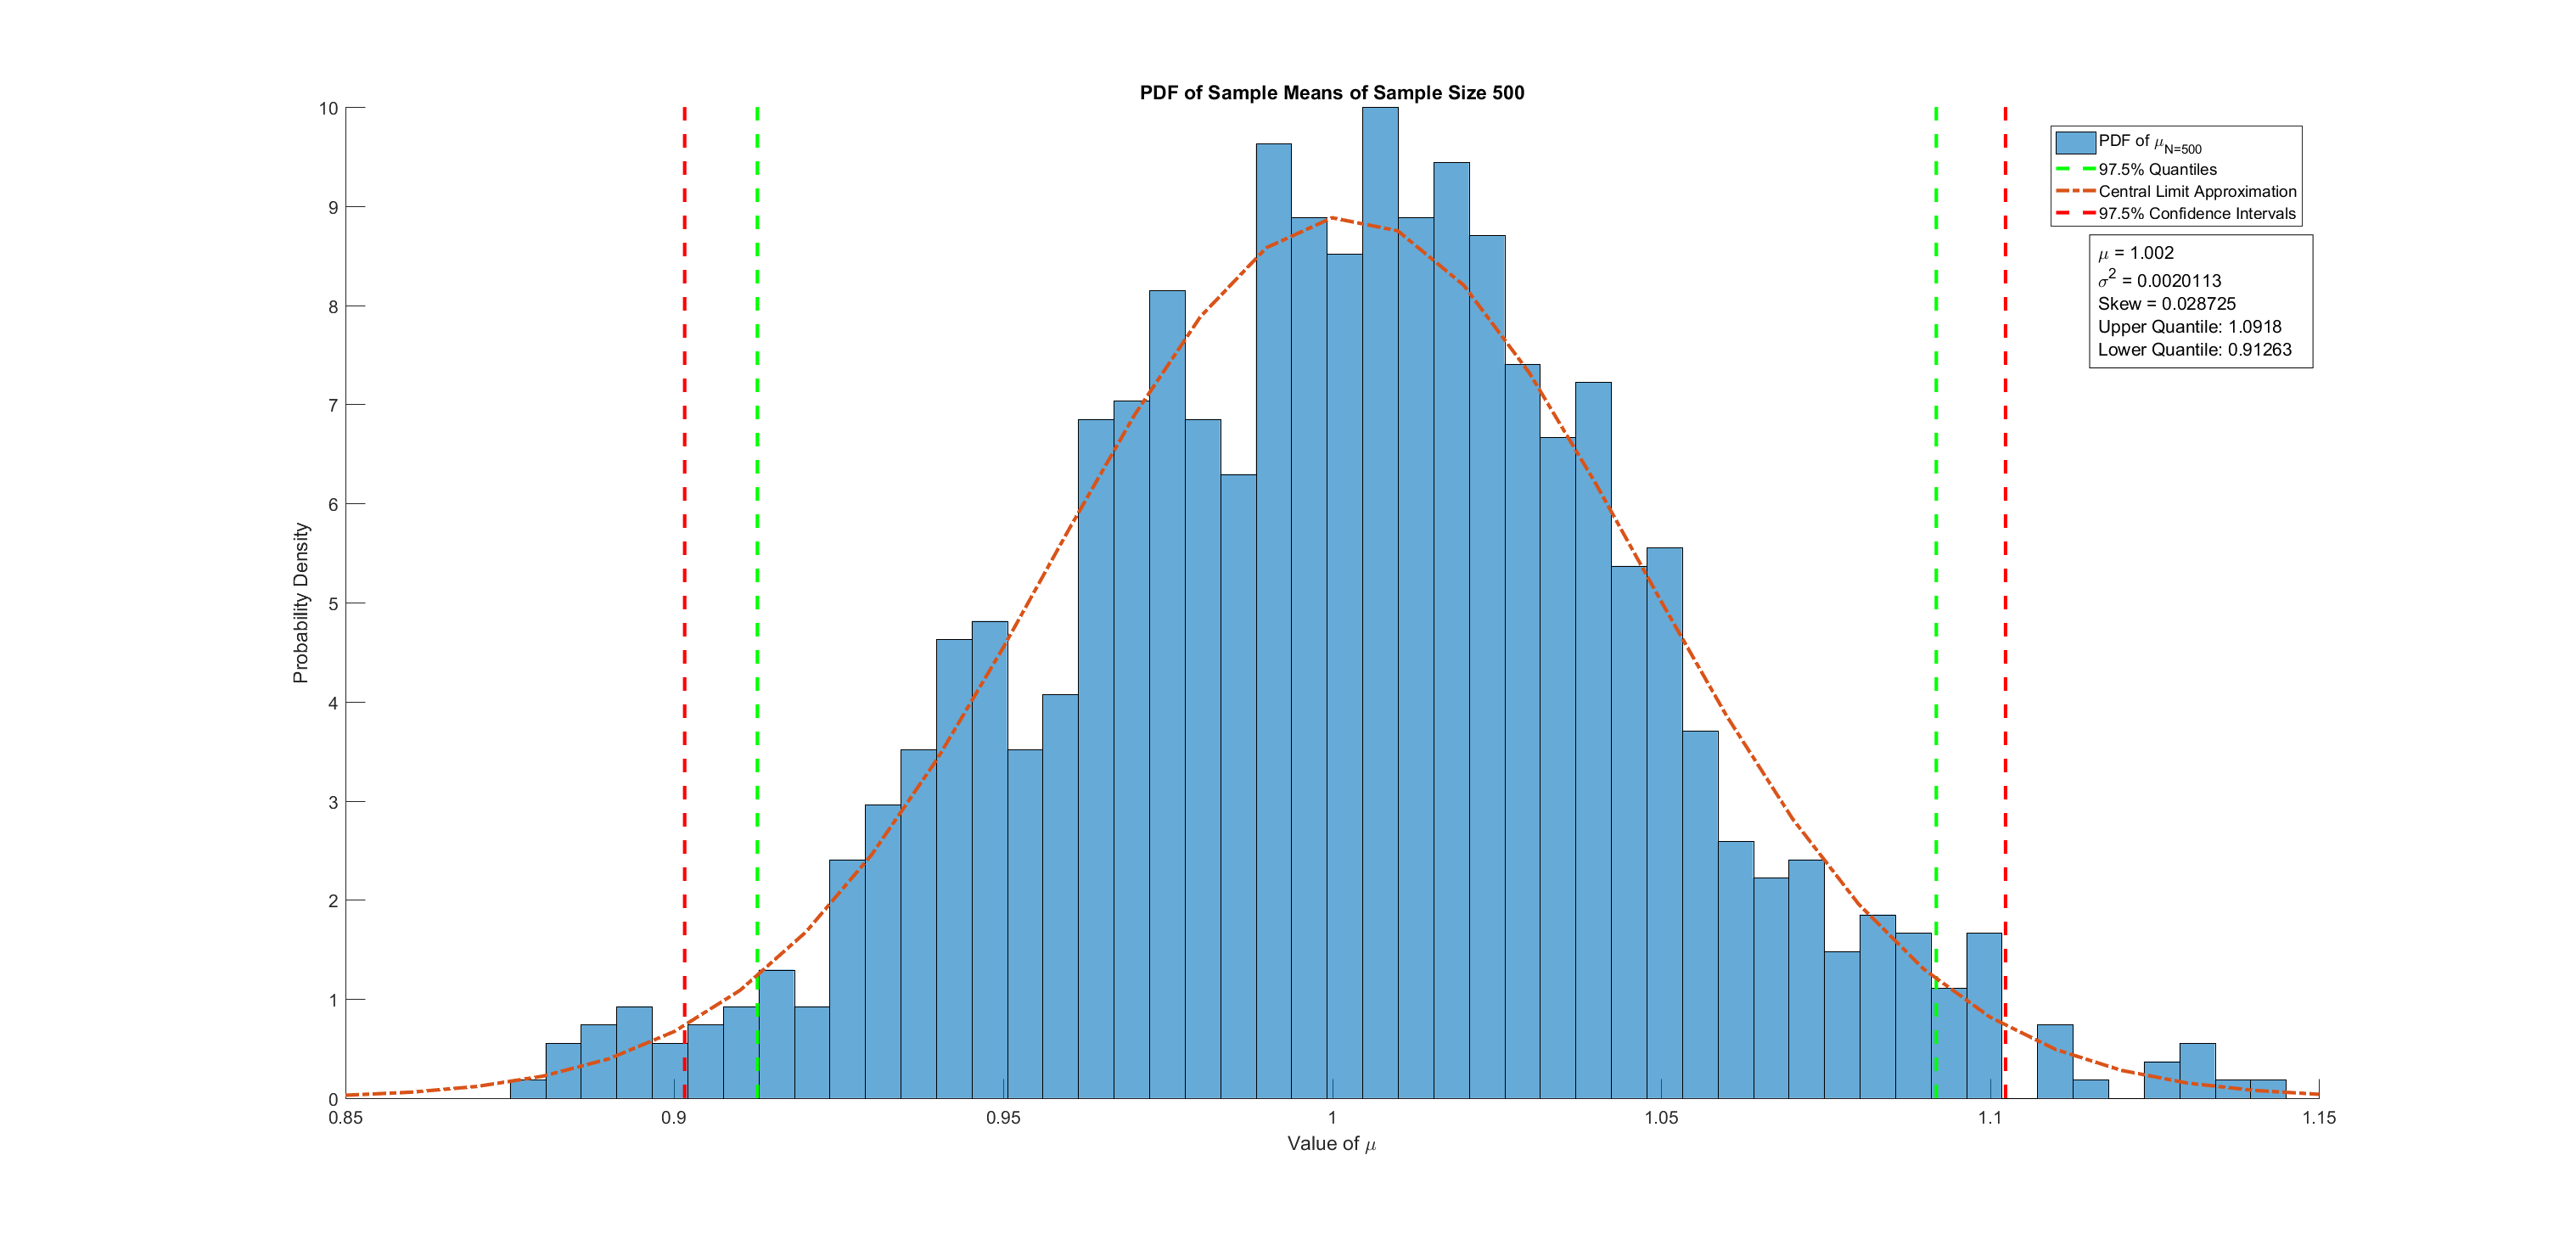
\includegraphics [width=\textwidth]{prob4_08.eps}

\end{document}
